\documentclass[12pt, oneside, a4paper]{book}
%\documentclass[12pt, a4paper]{book}
%----- 定義使用的 packages ----------------------

\usepackage{fontspec} 										% Font selection for XeLaTeX; see fontspec.pdf for documentation. 
\usepackage{xeCJK}											% 中文使用 XeCJK,但利用 \setCJKmainfont 定義粗體與斜體的字型
\defaultfontfeatures{Mapping=tex-text} 				% to support TeX conventions like ``---''
\usepackage{xunicode} 										% Unicode support for LaTeX character names (accents, European chars, etc)
\usepackage{xltxtra} 											% Extra customizations for XeLaTeX
\usepackage[sf,small]{titlesec}
\usepackage{amsmath, amssymb}
\usepackage{amsthm}										% theroemstyle 需要使用的套件
\usepackage{bm}                                                 % 排版粗體數學符號
\usepackage{enumerate}
\usepackage{graphicx, subfig, float} 					% support the \includegraphics command and options
\usepackage{array}
\usepackage{color, xcolor}
\usepackage{longtable, lscape}                                   % 跨頁的超長表格;lscape是旋轉此類表格的
\usepackage{threeparttable}                                     % 巨集,使表格加註解更容易(手冊p169)
\usepackage{multirow, booktabs}                                   % 讓表格編起來更美的套件(手冊p166),編輯跨列標題重覆的表格(手冊p182)
\usepackage{colortbl}                          				%.............................................表格標題註解之巨集套件
\usepackage{natbib}											% for Reference
\usepackage{makeidx}										% for Indexing
\usepackage[parfill]{parskip} % Activate to begin paragraphs with an empty line rather than an indent
%\usepackage{geometry} % See geometry.pdf to learn the layout options. There are lots.
%\usepackage[left=1.5in,right=1in,top=1in,bottom=1in]{geometry} 
\usepackage{url}                                                % 文稿內徵引網址
    \def\UrlFont{\rm}                                           % 網頁
\usepackage{fancyhdr}
	\pagestyle{fancy}
	\fancyhf{}                                     % 清除所有頁眉頁足
	\renewcommand{\headrulewidth}{0pt}                              % 頁眉下方的橫線    
%-----------------------------------------------------------------------------------------------------------------------
%  主字型設定
\setCJKmainfont
	[
		BoldFont=Heiti TC Medium								% 定義粗體的字型(依使用的電腦安裝的字型而定)
	]
	{cwTeX Q Ming Medium} 										% 設定中文內文字型
%	{新細明體}	
\setmainfont{Times New Roman}								% 設定英文內文字型
\setsansfont{Arial}														% used with {\sffamily ...}
%\setsansfont[Scale=MatchLowercase,Mapping=tex-text]{Gill Sans}
\setmonofont{Courier New}										% used with {\ttfamily ...}
%\setmonofont[Scale=MatchLowercase]{Andale Mono}
% 其他字型(隨使用的電腦安裝的字型不同,用註解的方式調整(打開或關閉))
% 英文字型
\newfontfamily{\E}{Cambria}										% 套用在內文中所有的英文字母
\newfontfamily{\A}{Arial}
\newfontfamily{\C}[Scale=0.9]{Cambria}
\newfontfamily{\T}{Times New Roman}
\newfontfamily{\TT}[Scale=0.8]{Times New Roman}
% 中文字型
\newCJKfontfamily{\MB}{微軟正黑體}							% 適用在 Mac 與 Win
\newCJKfontfamily{\SM}[Scale=0.8]{新細明體}				% 縮小版
%\newCJKfontfamily{\K}{標楷體}                        			% Windows 下的標楷體
\newCJKfontfamily{\K}{Kaiti TC Regular}         			% Mac OS 下的標楷體
\newCJKfontfamily{\BM}{Heiti TC Medium}					% Mac OS 下的黑體(粗體)
\newCJKfontfamily{\SR}{Songti TC Regular}				% Mac OS 下的宋體
\newCJKfontfamily{\SB}{Songti TC Bold}					% Mac OS 下的宋體(粗體)
\newCJKfontfamily{\CF}{cwTeX Q Fangsong Medium}	% CwTex 仿宋體
\newCJKfontfamily{\CB}{cwTeX Q Hei Bold}				% CwTex 粗黑體
\newCJKfontfamily{\CK}{cwTeX Q Kai Medium}   		% CwTex 楷體
\newCJKfontfamily{\CM}{cwTeX Q Ming Medium}		% CwTex 明體
\newCJKfontfamily{\CR}{cwTeX Q Yuan Medium}		% CwTex 圓體
%-----------------------------------------------------------------------------------------------------------------------
\XeTeXlinebreaklocale "zh"                  				%這兩行一定要加,中文才能自動換行
\XeTeXlinebreakskip = 0pt plus 1pt     %這兩行一定要加,中文才能自動換行
%-----------------------------------------------------------------------------------------------------------------------
%----- 重新定義的指令 ---------------------------
\newcommand{\cw}{\texttt{cw}\kern-.6pt\TeX}	% 這是 cwTex 的 logo 文字
\newcommand{\imgdir}{graph/}							% 設定圖檔的位置
\renewcommand{\tablename}{表}						% 改變表格標號文字為中文的「表」(預設為 Table)
\renewcommand{\figurename}{圖}						% 改變圖片標號文字為中文的「圖」(預設為 Figure)
\renewcommand{\contentsname}{目~錄}
\renewcommand\listfigurename{圖目錄}
\renewcommand\listtablename{表目錄}
\renewcommand{\appendixname}{附~錄}                  
\renewcommand{\indexname}{索引}
\renewcommand{\bibname}{參考文獻}
%-----------------------------------------------------------------------------------------------------------------------

\theoremstyle{plain}
\newtheorem{de}{Definition}[section]				%definition獨立編號
\newtheorem{thm}{定理}[section]			%theorem 獨立編號,取中文名稱並給予不同字型
\newtheorem{lemma}[thm]{引理}				%lemma 與 theorem 共用編號
\newtheorem{ex}{{\E Example}}						%example 獨立編號,不編入小節數字,走流水號。也換個字型。
\newtheorem{cor}{Corollary}[section]				%not used here
\newtheorem{exercise}{EXERCISE}					%not used here
\newtheorem{re}{\emph{Result}}[section]		%not used here
\newtheorem{axiom}{AXIOM}							%not used here
\renewcommand{\proofname}{\textbf{Proof}}		%not used here

\newcommand{\loflabel}{圖} % 圖目錄出現 圖 x.x 的「圖」字
\newcommand{\lotlabel}{表}  % 表目錄出現 表 x.x 的「表」字

\parindent=0pt

%--- 其他定義 ----------------------------------
% 定義章節標題的字型、大小
\titleformat{\chapter}[display]{\raggedleft\LARGE\bfseries\CF}		% 定義章抬頭靠右(\reggedleft)
 { 第\ \thechapter\ 章}{0.2cm}{}
%\titleformat{\chapter}[hang]{\centering\LARGE\sf}{\MB 第~\thesection~章}{0.2cm}{}%控制章的字體
%\titleformat{\section}[hang]{\Large\sf}{\MB 第~\thesection~節}{0.2cm}{}%控制章的字體
%\titleformat{\subsection}[hang]{\centering\Large\sf}{\MB 第~\thesubsection~節}{0.2cm}{}%控制節的字體
%\titleformat*{\section}{\normalfont\Large\bfseries\MB}
%\titleformat*{\subsection}{\normalfont\large\bfseries\MB}
%\titleformat*{\subsubsection}{\normalfont\large\bfseries\MB}


% 顏色定義
\definecolor{heavy}{gray}{.9}								% 0.9深淺度之灰色
\definecolor{light}{gray}{.8}
\definecolor{pink}{rgb}{0.99,0.91,0.95}               % 定義pink顏色

\usepackage{wallpaper}                                          % 使用浮水印
\CenterWallPaper{0.6}{graph/ntpu.eps}                           % 浮水印圖檔

%--- 製作封面頁 ----------------------------------
\begin{document}
\fontsize{12}{22pt}\selectfont
 \begin{center}
    \huge 國立台北大學統計學系 \\ 碩士論文
 \end{center}
\vspace*{2cm}
 \begin{center}
    \LARGE 指導教授: 黃怡婷~~博士 \\
 \end{center}
\vspace*{2cm}
 \begin{center}
    \LARGE 建構多變量二元聯合機率分配並應用於長期追蹤資料模型\\
         Building the Multivariate Joint Distribution for Binary Data and its Application in Longitudinal Marginal Model
 \end{center}
\vspace*{5cm}
\begin{center}
    \LARGE 研究生:葉麗芬 \\
    \LARGE 中華民國~一$\bigcirc$三~年~七~月
\end{center}

\newpage
%\input{preambleforpaper}
%\title{}
%\date{}
%\author{}
%\begin{document}

\chead{\LARGE 謝~誌}
謹以此檔案,感謝 台北大學統計學系在我求學期間的照顧, 黃怡婷老師及 汪群超老師對我的指導,當然還要謝謝支持我逐夢的家人朋友。
希望這些從所撰論文截取出的 \cw 編輯技巧,能對撰寫論文中的學弟妹們有所幫助,也祝福你在接下來的寫作過程順利。

\vspace*{10cm}

\begin{flushright}
葉麗芬 謹誌于 \\
中華民國~一$\bigcirc$三~年~七~月
\end{flushright}

%\end{document}   		% 謝誌
%\documentclass[12pt]{article}
%\usepackage{fancyhdr}
%\usepackage{indentfirst}
%
%\begin{document}
%\fontsize{12}{20pt}\selectfont
\fancyhf{}
\begin{center}
{\large 國立台北大學一$\bigcirc$二學年度第二學期碩士學位論文提要}
\fboxrule=1pt
\fboxsep=20pt
\fbox{\begin{minipage}{12cm}
\noindent 論文題目:~\underline{~~建構多變量二元聯合機率分配並應用於長期追蹤資料模型~~}

\noindent 論文頁數:~\underline{~~~85~~~}

\noindent 所~組~別:~\underline{~~統計學系碩士班~~}~~系(所)~~\underline{~~~~~~~~}~組~(學號:~\underline{~~710133121}~~)

\noindent 研~究~生:~\underline{~~~~~~葉麗芬~~~~~}~~指導教授:~\underline{~~~~黃怡婷~~~~}

\bigskip
\noindent 論文提要內容:

\qquad 現今許多科學研究常藉由觀察相同群體多個時間點的狀況來了解所關心事件對此群體所產生的長期平均影響,
這類型研究需要使用長期追蹤資料分析方法來瞭解影響平均反應趨勢的變數,以供後續決策或研究參考。

\qquad 在一階馬可夫鏈 (First-Order Markov Chains) 的假設下,本論文利用 Biswas 和 Hwang (2002) 提出之二元二項分配 (Bivariate Binomial Distribution) 建構出多變量聯合二元機率
分配,並討論該分配的特性,推導參數的最大概似估計式,及其大樣本性質。藉由此多變量分配,本論文提出利用最大概似估計法來估計長期追蹤資料之廣義線性模型中參數,
最後運用統計模擬來探討新的多變量二元聯合機率分配參數與長期追蹤資料之廣義線性模型參數的最大概似估計式表現,再與現行研究者常採用的廣義估計方程式的參數估計方法進行比較。

\vspace*{2cm}
\noindent 關鍵詞: 二元長期追蹤資料、多變量二元分配、長期追蹤資料的廣義線性模型、最大概似估計法
\medskip
\end{minipage}}
\end{center}

%%%%%%%%%%%%%%%%%%%%%%%%%%%% ABSTRACT %%%%%%%%%%%%%%%%%%%%%%%%%%%%%%%%%%%%%%%%%%%%%
\newpage
\thispagestyle{empty}
\fontsize{12}{18pt}\selectfont

\begin{center}{\Large \bf ABSTRACT}\\[20pt]
    {\large Building the Multivariate Joint Distribution for Binary Data and its Application in Longitudinal Marginal Model}\\[10pt]
        by\\[10pt]  YE,\,LI-FEN\\[10pt] July 2014
\end{center}
{\small ADVISOR: Dr. HWANG, YI-TING \\[5pt]
        DEPARTMENT: DEPARTMENT OF STATISTICS\\[5pt]
        MAJOR: STATISTICS\\[5pt]
        DEGREE: MASTER OF SCIENCE}\\[10pt]
\noindent
Many recent studies often observe the response variables repeatedly to understand the influence of certain conditions longitudinally.
The general linear model and generalized linear model for longitudinal data are used to make inference of this kind of data.
Since the response variable is observed repeatedly, the model settings and estimations would need the multivariate distribution.
Many continuous multivariate distributions have been proposed in the literatures.
However, owing to the complexity of describing the association among the multivariate discrete random variables, it is lack of the well-known distribution.
To estimate the parameter in the generalized linear model for longitudinal data, the generalized estimating equation (GEE) proposed by Liang and Zeger (1986) is a commonly used estimating method.

\vspace*{2cm}
\noindent {\scshape KEY WORDS}: Binary Longitudinal Data, Multivariate Binomial Distribution, Marginal Model, Maximum Likelihood Estimation.
%\end{document}

   	% 中英文摘要

%%%%%%%%%%%%%%%%%%%%%%%%%% 製作目錄 %%%%%%%%%%%%%%%%%%%%%%%%%%%%%%%%%%%%%%
\newpage					
\fontsize{12}{22pt}\selectfont 	% 字型大小與行距視使用的字型調整
\fancyfoot[C]{\thepage}

\setcounter{tocdepth}{2}		% 目錄層次
\pagenumbering{roman}			% 羅馬文頁碼
\tableofcontents
\newpage
\renewcommand{\numberline}[1]{\loflabel~#1\hspace*{1em}}% 圖目錄出現 圖 x.x 的「圖」字
\listoffigures %圖目錄
\newpage
\renewcommand{\numberline}[1]{\lotlabel~#1\hspace*{1em}}% 表目錄出現 表 x.x 的「表」字
\listoftables % 表目錄

%%%%%%%%%%%%%%%%%%%%%%%%% 正文開始 %%%%%%%%%%%%%%%%%%%%%%%%%%%%%%%%%%%%%%
\cleardoublepage
\pagenumbering{arabic}          % 重新開始計算頁碼-格式阿拉伯文
\setcounter{page}{1}
%\documentclass[12pt, oneside, a4paper]{book}
%\documentclass[12pt, a4paper]{book}
%----- 定義使用的 packages ----------------------

\usepackage{fontspec} 										% Font selection for XeLaTeX; see fontspec.pdf for documentation. 
\usepackage{xeCJK}											% 中文使用 XeCJK,但利用 \setCJKmainfont 定義粗體與斜體的字型
\defaultfontfeatures{Mapping=tex-text} 				% to support TeX conventions like ``---''
\usepackage{xunicode} 										% Unicode support for LaTeX character names (accents, European chars, etc)
\usepackage{xltxtra} 											% Extra customizations for XeLaTeX
\usepackage[sf,small]{titlesec}
\usepackage{amsmath, amssymb}
\usepackage{amsthm}										% theroemstyle 需要使用的套件
\usepackage{bm}                                                 % 排版粗體數學符號
\usepackage{enumerate}
\usepackage{graphicx, subfig, float} 					% support the \includegraphics command and options
\usepackage{array}
\usepackage{color, xcolor}
\usepackage{longtable, lscape}                                   % 跨頁的超長表格;lscape是旋轉此類表格的
\usepackage{threeparttable}                                     % 巨集,使表格加註解更容易(手冊p169)
\usepackage{multirow, booktabs}                                   % 讓表格編起來更美的套件(手冊p166),編輯跨列標題重覆的表格(手冊p182)
\usepackage{colortbl}                          				%.............................................表格標題註解之巨集套件
\usepackage{natbib}											% for Reference
\usepackage{makeidx}										% for Indexing
\usepackage[parfill]{parskip} % Activate to begin paragraphs with an empty line rather than an indent
%\usepackage{geometry} % See geometry.pdf to learn the layout options. There are lots.
%\usepackage[left=1.5in,right=1in,top=1in,bottom=1in]{geometry} 
\usepackage{url}                                                % 文稿內徵引網址
    \def\UrlFont{\rm}                                           % 網頁
\usepackage{fancyhdr}
	\pagestyle{fancy}
	\fancyhf{}                                     % 清除所有頁眉頁足
	\renewcommand{\headrulewidth}{0pt}                              % 頁眉下方的橫線    
%-----------------------------------------------------------------------------------------------------------------------
%  主字型設定
\setCJKmainfont
	[
		BoldFont=Heiti TC Medium								% 定義粗體的字型(依使用的電腦安裝的字型而定)
	]
	{cwTeX Q Ming Medium} 										% 設定中文內文字型
%	{新細明體}	
\setmainfont{Times New Roman}								% 設定英文內文字型
\setsansfont{Arial}														% used with {\sffamily ...}
%\setsansfont[Scale=MatchLowercase,Mapping=tex-text]{Gill Sans}
\setmonofont{Courier New}										% used with {\ttfamily ...}
%\setmonofont[Scale=MatchLowercase]{Andale Mono}
% 其他字型(隨使用的電腦安裝的字型不同,用註解的方式調整(打開或關閉))
% 英文字型
\newfontfamily{\E}{Cambria}										% 套用在內文中所有的英文字母
\newfontfamily{\A}{Arial}
\newfontfamily{\C}[Scale=0.9]{Cambria}
\newfontfamily{\T}{Times New Roman}
\newfontfamily{\TT}[Scale=0.8]{Times New Roman}
% 中文字型
\newCJKfontfamily{\MB}{微軟正黑體}							% 適用在 Mac 與 Win
\newCJKfontfamily{\SM}[Scale=0.8]{新細明體}				% 縮小版
%\newCJKfontfamily{\K}{標楷體}                        			% Windows 下的標楷體
\newCJKfontfamily{\K}{Kaiti TC Regular}         			% Mac OS 下的標楷體
\newCJKfontfamily{\BM}{Heiti TC Medium}					% Mac OS 下的黑體(粗體)
\newCJKfontfamily{\SR}{Songti TC Regular}				% Mac OS 下的宋體
\newCJKfontfamily{\SB}{Songti TC Bold}					% Mac OS 下的宋體(粗體)
\newCJKfontfamily{\CF}{cwTeX Q Fangsong Medium}	% CwTex 仿宋體
\newCJKfontfamily{\CB}{cwTeX Q Hei Bold}				% CwTex 粗黑體
\newCJKfontfamily{\CK}{cwTeX Q Kai Medium}   		% CwTex 楷體
\newCJKfontfamily{\CM}{cwTeX Q Ming Medium}		% CwTex 明體
\newCJKfontfamily{\CR}{cwTeX Q Yuan Medium}		% CwTex 圓體
%-----------------------------------------------------------------------------------------------------------------------
\XeTeXlinebreaklocale "zh"                  				%這兩行一定要加,中文才能自動換行
\XeTeXlinebreakskip = 0pt plus 1pt     %這兩行一定要加,中文才能自動換行
%-----------------------------------------------------------------------------------------------------------------------
%----- 重新定義的指令 ---------------------------
\newcommand{\cw}{\texttt{cw}\kern-.6pt\TeX}	% 這是 cwTex 的 logo 文字
\newcommand{\imgdir}{graph/}							% 設定圖檔的位置
\renewcommand{\tablename}{表}						% 改變表格標號文字為中文的「表」(預設為 Table)
\renewcommand{\figurename}{圖}						% 改變圖片標號文字為中文的「圖」(預設為 Figure)
\renewcommand{\contentsname}{目~錄}
\renewcommand\listfigurename{圖目錄}
\renewcommand\listtablename{表目錄}
\renewcommand{\appendixname}{附~錄}                  
\renewcommand{\indexname}{索引}
\renewcommand{\bibname}{參考文獻}
%-----------------------------------------------------------------------------------------------------------------------

\theoremstyle{plain}
\newtheorem{de}{Definition}[section]				%definition獨立編號
\newtheorem{thm}{定理}[section]			%theorem 獨立編號,取中文名稱並給予不同字型
\newtheorem{lemma}[thm]{引理}				%lemma 與 theorem 共用編號
\newtheorem{ex}{{\E Example}}						%example 獨立編號,不編入小節數字,走流水號。也換個字型。
\newtheorem{cor}{Corollary}[section]				%not used here
\newtheorem{exercise}{EXERCISE}					%not used here
\newtheorem{re}{\emph{Result}}[section]		%not used here
\newtheorem{axiom}{AXIOM}							%not used here
\renewcommand{\proofname}{\textbf{Proof}}		%not used here

\newcommand{\loflabel}{圖} % 圖目錄出現 圖 x.x 的「圖」字
\newcommand{\lotlabel}{表}  % 表目錄出現 表 x.x 的「表」字

\parindent=0pt

%--- 其他定義 ----------------------------------
% 定義章節標題的字型、大小
\titleformat{\chapter}[display]{\raggedleft\LARGE\bfseries\CF}		% 定義章抬頭靠右(\reggedleft)
 { 第\ \thechapter\ 章}{0.2cm}{}
%\titleformat{\chapter}[hang]{\centering\LARGE\sf}{\MB 第~\thesection~章}{0.2cm}{}%控制章的字體
%\titleformat{\section}[hang]{\Large\sf}{\MB 第~\thesection~節}{0.2cm}{}%控制章的字體
%\titleformat{\subsection}[hang]{\centering\Large\sf}{\MB 第~\thesubsection~節}{0.2cm}{}%控制節的字體
%\titleformat*{\section}{\normalfont\Large\bfseries\MB}
%\titleformat*{\subsection}{\normalfont\large\bfseries\MB}
%\titleformat*{\subsubsection}{\normalfont\large\bfseries\MB}


% 顏色定義
\definecolor{heavy}{gray}{.9}								% 0.9深淺度之灰色
\definecolor{light}{gray}{.8}
\definecolor{pink}{rgb}{0.99,0.91,0.95}               % 定義pink顏色

%\title{第1章 \\ 緒~論}
%\date{}
%\author{}
%\begin{document}
%\maketitle

\chapter{緒~論}
現今許多科學研究藉由分析相同群體在多個時間點的狀況,來衡量所關心之事件對此群體所產生的長期趨勢影響。例如:流行病學家想找出某項疾病之致病基因,
醫生或藥廠想知道某藥物或療法對病人的治療效果,證券分析師想研究某產業下之公司近年的經營狀況$\cdots\cdots$等。
此類型資料因同時具有時間序列(Time Series)與橫斷面(Cross Section)訊息,所提供的訊息較單一層面資料更為充份完整,故不管是在生物醫藥科技、商業行為、或是公共政策研究領域,
收集此類型資料進行分析之研究與日俱增。然在流行病學、遺傳醫學等健康相關研究領域稱此為長期追蹤資料(Longitudinal Data);而在財務金融、計量經濟等商業相關研究領域,
則稱之為縱橫斷面資料(Panel Data)。

分析長期追蹤資料時,若反應變數為連續型或二元資料時,常會繪製反應變數的平均反應曲線(Mean Response Curve),以便初步了解平均反應隨時間而變化的軌跡。
圖 \ref{fig:meancurve} 係以兩個長期追蹤資料為例繪製的平均反應曲線,圖 \ref{fig:meancurve}\subref{fig:a} 為研究者想了解4種不同飼養策略,是否影響實驗室老鼠在實驗期間
體重增加之趨勢,故分別在實驗的一開始(第0週)及後續的第1, 2, 4, 8, 12週測量老鼠的體重,屬連續型長期追蹤資料;
圖 \ref{fig:meancurve}\subref{fig:b} 則為二元(Binary)長期追蹤資料,係臨床研究者想了解某種積極治療法是否可改善患有呼吸上疾病病人之呼吸狀態,此研究採隨機指派方式決定病人接受的治療為積極治療法或是安慰劑(Placebo)治療,
病人每週回診1次,共回診4次,紀錄呼吸狀態有改善者為1,未改善者為0,以計算、分析改善比率。

\begin{figure}[h]
    \centering
       \subfloat[連續型資料實例:不同飼養策略對實驗室老鼠於實驗期間體重增加趨勢之影響]{\label{fig:a}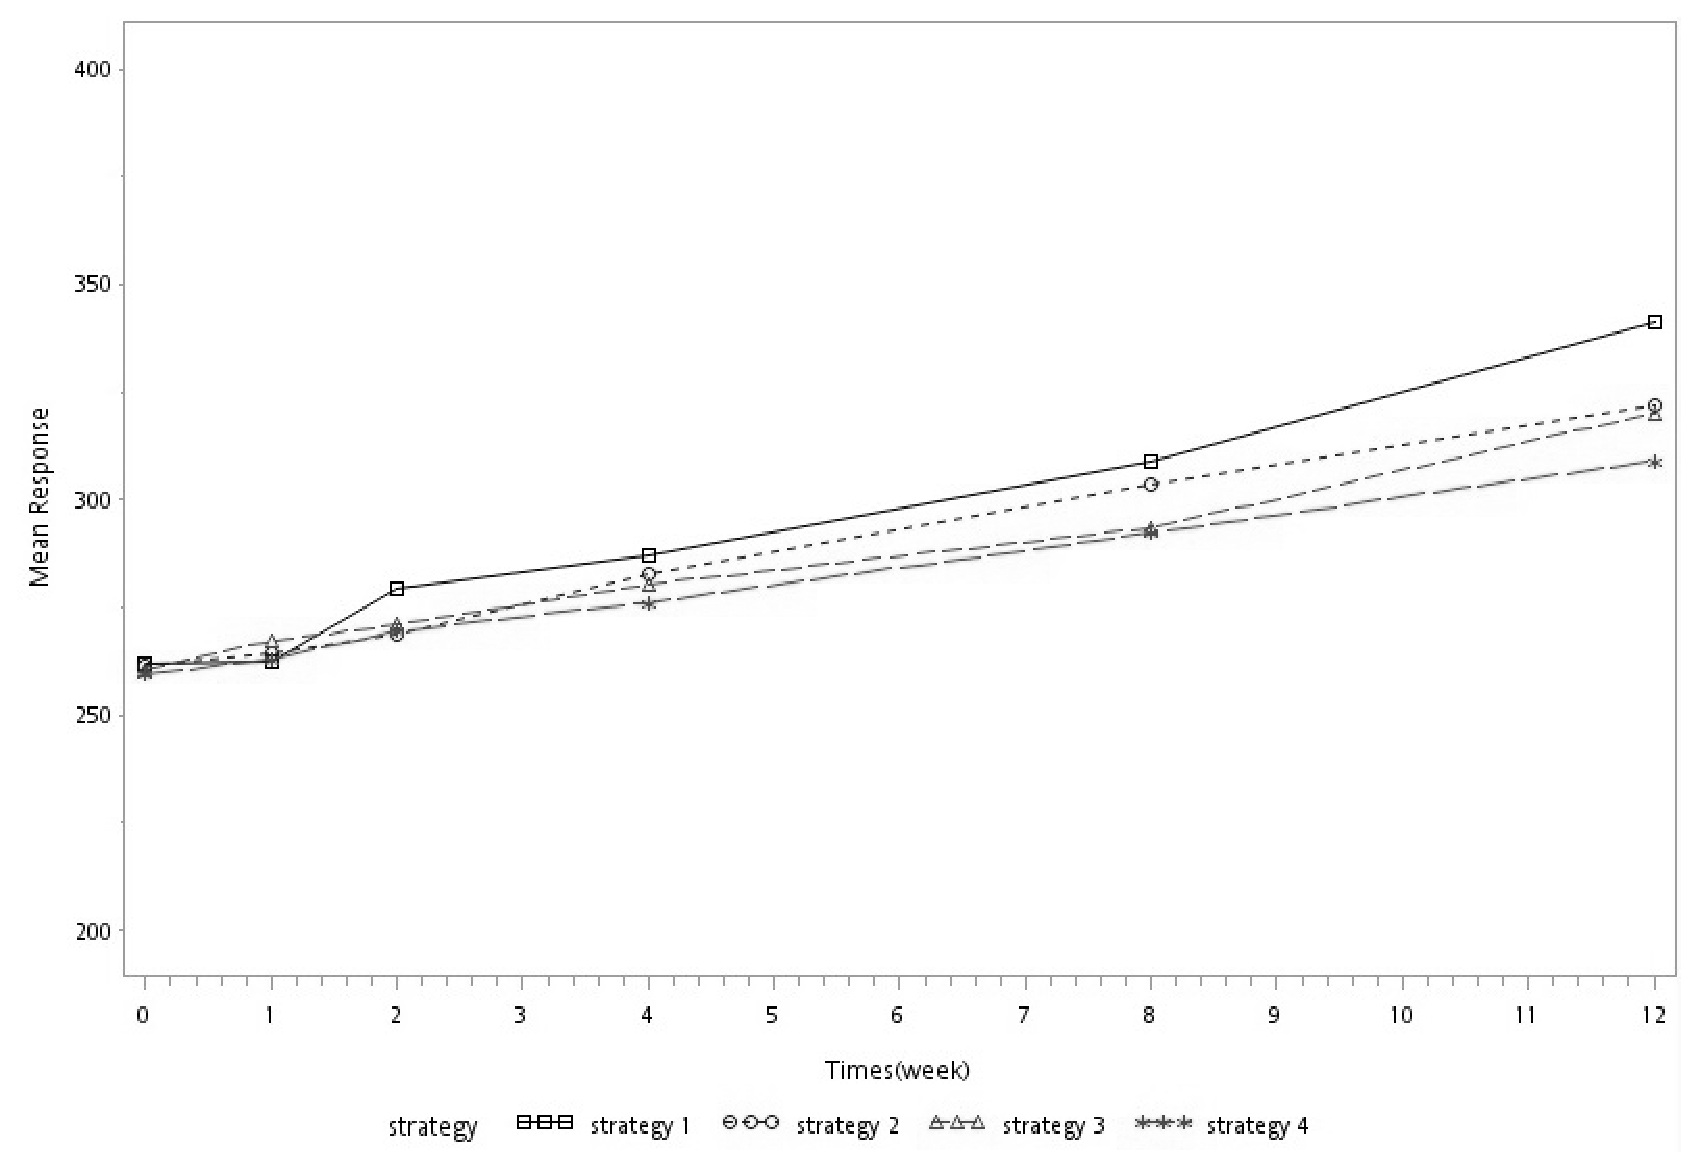
\includegraphics[height=7cm,width=0.8\textwidth]{graph/la_p4_sp5.eps}}\\
       \subfloat[類別型資料實例:不同治療方法是否改變患有呼吸上疾病病人呼吸狀態研究之改善比率曲線]{\label{fig:b}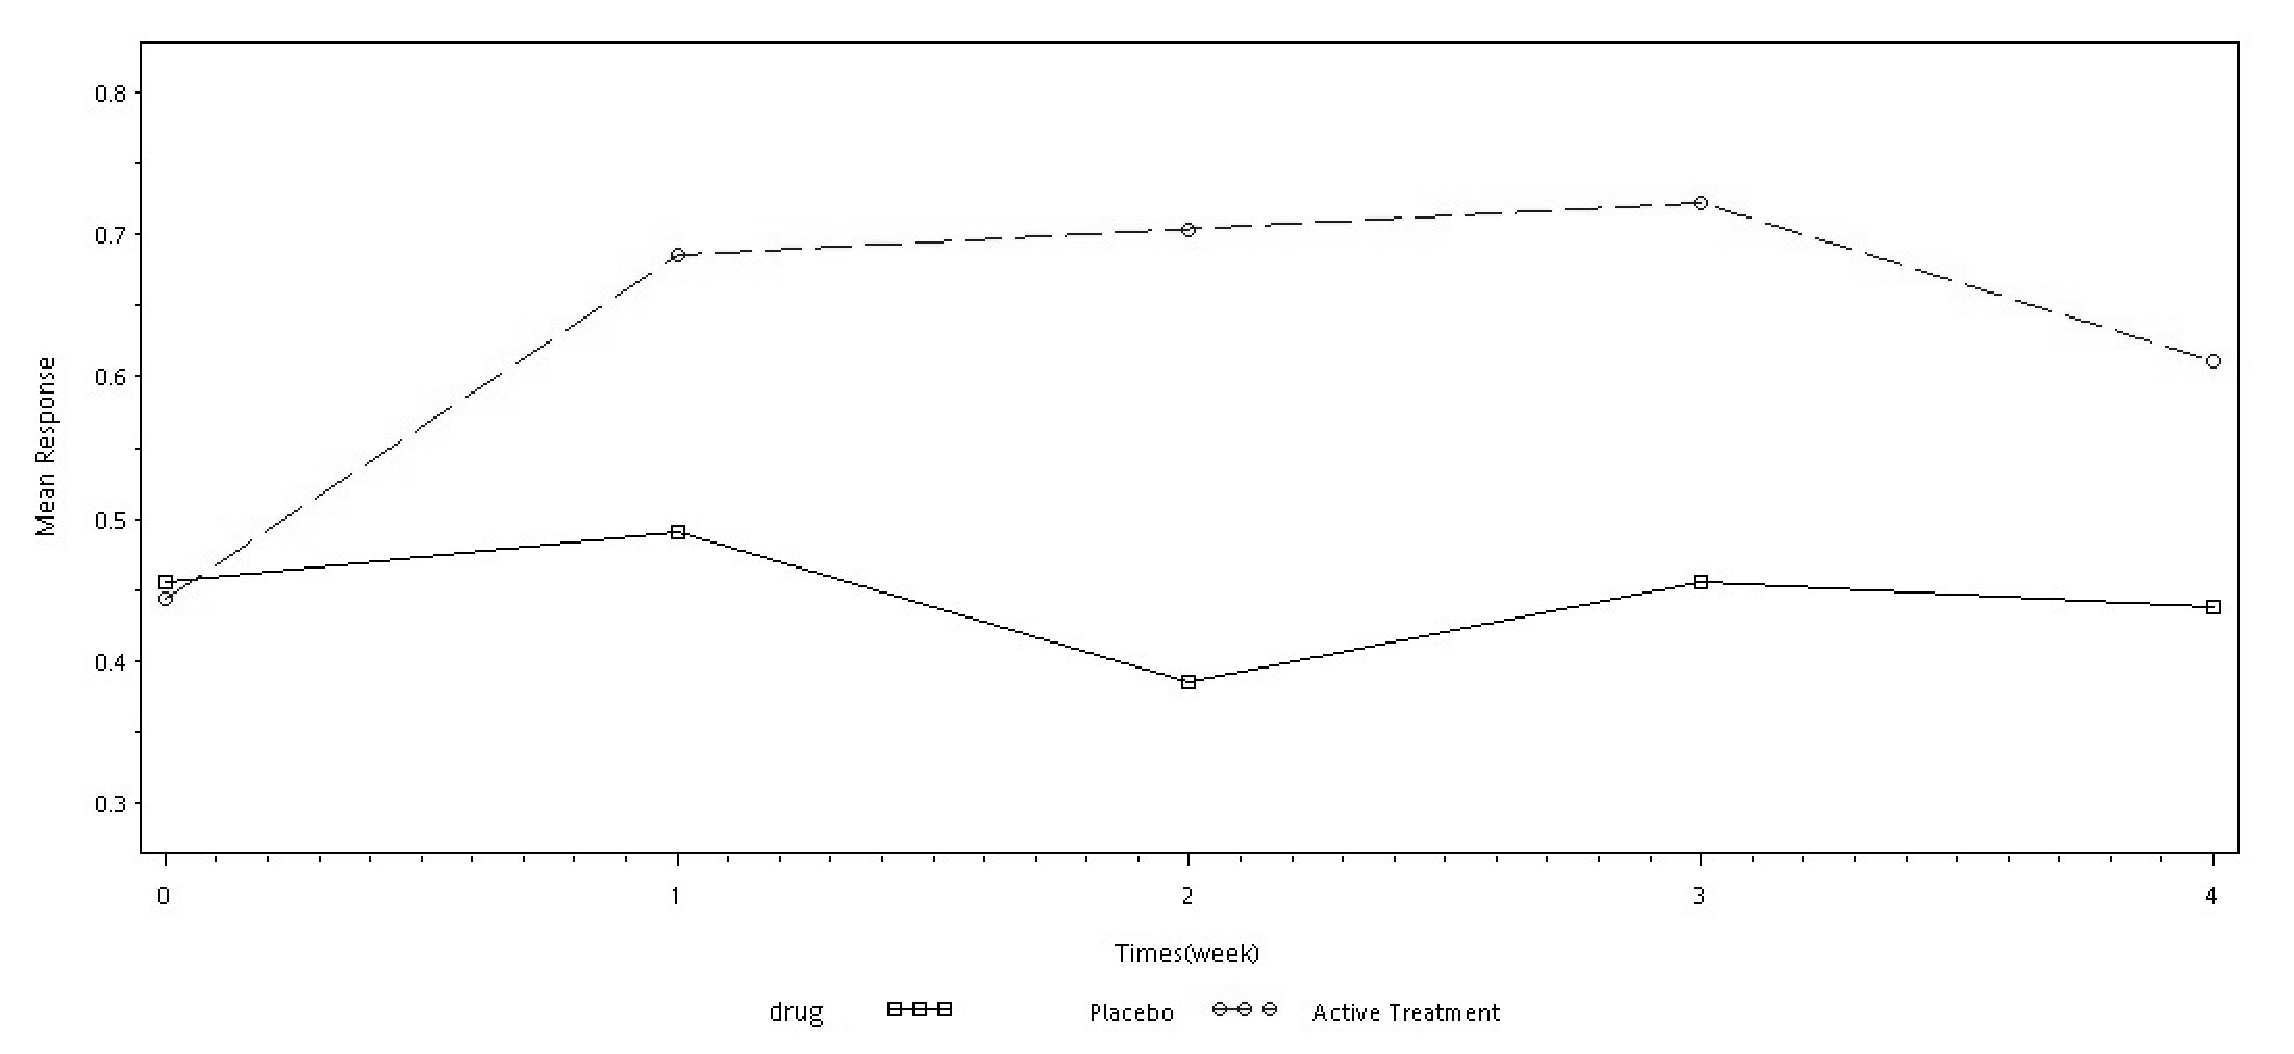
\includegraphics[height=7cm,width=0.8\textwidth]{graph/p6_1.eps}}
       \caption{長期追蹤資料平均反應曲線}
    \label{fig:meancurve}
\end{figure}

此外,藉由反應變數之共變異數矩陣(Covariance Matrix)來了解同一研究對象各次試驗結果間的關係。
令 $\sigma_{tu}$ 代表時間點 $t$ 與 $u$ 試驗結果的共變異數, $t,u=1,\ldots,k$, 並將第 $i$ 個研究對象之共變異數矩陣表示如下:
$$\mbox{Cov}(\bm{Y}_i)=\left(
            \begin{array}{cccc}
             \sigma_{11}     &\sigma_{12}    &\cdots &\sigma_{1k} \\
             \sigma_{21}    &\sigma_{22}     &\cdots &\sigma_{2k} \\
             \vdots         &\vdots         &\ddots &\vdots  \\
             \sigma_{k1}    &\sigma_{k2}    &\cdots &\sigma_{kk}
            \end{array} \right),$$
在分析資料時,共變異數矩陣可以假設與研究個體 $i$ 有關,但一般實務上研究個數在同一時間點通常不會有重覆測量的資料,故為簡化以下討論,本論文假設每一研究對象均有相同共變異數結構。
由於生物性,長期追蹤資料之關係隨著間隔時間的增加而遞減,且試驗結果間會有正相關,故在資料分析時多會針對各試驗時間點資料間之共變異數模型(Covariance Pattern)進行假設。

本論文將在第~ \ref{ch:dist} ~章說明多變量二元聯合機率分配的建構概念及此分配的特性;
第~ \ref{ch:model} ~章介紹二元長期追蹤資料如何以邊際模型配適平均反應模型;
第~ \ref{ch:simu} ~章為數值模擬分析結果,包括多變量二元分配在不同樣本和參數假設下之參數估計結果比較,及在不同資料型態和工作矩陣假設下,二種平均反應模型之參數估計結果比較;
最後,在第~ \ref{ch:final} ~章總結本研究的結果,並對本論文所建立的分析方法及後續研究提出建議。

%\end{document}


             % CH1: introduction
\ifodd\count0 \else \thispagestyle{empty}\mbox{}\clearpage\fi % 如果是偶數頁就呈現空白頁
%\documentclass[12pt, oneside, a4paper]{book}
%\documentclass[12pt, a4paper]{book}
%----- 定義使用的 packages ----------------------

\usepackage{fontspec} 										% Font selection for XeLaTeX; see fontspec.pdf for documentation. 
\usepackage{xeCJK}											% 中文使用 XeCJK,但利用 \setCJKmainfont 定義粗體與斜體的字型
\defaultfontfeatures{Mapping=tex-text} 				% to support TeX conventions like ``---''
\usepackage{xunicode} 										% Unicode support for LaTeX character names (accents, European chars, etc)
\usepackage{xltxtra} 											% Extra customizations for XeLaTeX
\usepackage[sf,small]{titlesec}
\usepackage{amsmath, amssymb}
\usepackage{amsthm}										% theroemstyle 需要使用的套件
\usepackage{bm}                                                 % 排版粗體數學符號
\usepackage{enumerate}
\usepackage{graphicx, subfig, float} 					% support the \includegraphics command and options
\usepackage{array}
\usepackage{color, xcolor}
\usepackage{longtable, lscape}                                   % 跨頁的超長表格;lscape是旋轉此類表格的
\usepackage{threeparttable}                                     % 巨集,使表格加註解更容易(手冊p169)
\usepackage{multirow, booktabs}                                   % 讓表格編起來更美的套件(手冊p166),編輯跨列標題重覆的表格(手冊p182)
\usepackage{colortbl}                          				%.............................................表格標題註解之巨集套件
\usepackage{natbib}											% for Reference
\usepackage{makeidx}										% for Indexing
\usepackage[parfill]{parskip} % Activate to begin paragraphs with an empty line rather than an indent
%\usepackage{geometry} % See geometry.pdf to learn the layout options. There are lots.
%\usepackage[left=1.5in,right=1in,top=1in,bottom=1in]{geometry} 
\usepackage{url}                                                % 文稿內徵引網址
    \def\UrlFont{\rm}                                           % 網頁
\usepackage{fancyhdr}
	\pagestyle{fancy}
	\fancyhf{}                                     % 清除所有頁眉頁足
	\renewcommand{\headrulewidth}{0pt}                              % 頁眉下方的橫線    
%-----------------------------------------------------------------------------------------------------------------------
%  主字型設定
\setCJKmainfont
	[
		BoldFont=Heiti TC Medium								% 定義粗體的字型(依使用的電腦安裝的字型而定)
	]
	{cwTeX Q Ming Medium} 										% 設定中文內文字型
%	{新細明體}	
\setmainfont{Times New Roman}								% 設定英文內文字型
\setsansfont{Arial}														% used with {\sffamily ...}
%\setsansfont[Scale=MatchLowercase,Mapping=tex-text]{Gill Sans}
\setmonofont{Courier New}										% used with {\ttfamily ...}
%\setmonofont[Scale=MatchLowercase]{Andale Mono}
% 其他字型(隨使用的電腦安裝的字型不同,用註解的方式調整(打開或關閉))
% 英文字型
\newfontfamily{\E}{Cambria}										% 套用在內文中所有的英文字母
\newfontfamily{\A}{Arial}
\newfontfamily{\C}[Scale=0.9]{Cambria}
\newfontfamily{\T}{Times New Roman}
\newfontfamily{\TT}[Scale=0.8]{Times New Roman}
% 中文字型
\newCJKfontfamily{\MB}{微軟正黑體}							% 適用在 Mac 與 Win
\newCJKfontfamily{\SM}[Scale=0.8]{新細明體}				% 縮小版
%\newCJKfontfamily{\K}{標楷體}                        			% Windows 下的標楷體
\newCJKfontfamily{\K}{Kaiti TC Regular}         			% Mac OS 下的標楷體
\newCJKfontfamily{\BM}{Heiti TC Medium}					% Mac OS 下的黑體(粗體)
\newCJKfontfamily{\SR}{Songti TC Regular}				% Mac OS 下的宋體
\newCJKfontfamily{\SB}{Songti TC Bold}					% Mac OS 下的宋體(粗體)
\newCJKfontfamily{\CF}{cwTeX Q Fangsong Medium}	% CwTex 仿宋體
\newCJKfontfamily{\CB}{cwTeX Q Hei Bold}				% CwTex 粗黑體
\newCJKfontfamily{\CK}{cwTeX Q Kai Medium}   		% CwTex 楷體
\newCJKfontfamily{\CM}{cwTeX Q Ming Medium}		% CwTex 明體
\newCJKfontfamily{\CR}{cwTeX Q Yuan Medium}		% CwTex 圓體
%-----------------------------------------------------------------------------------------------------------------------
\XeTeXlinebreaklocale "zh"                  				%這兩行一定要加,中文才能自動換行
\XeTeXlinebreakskip = 0pt plus 1pt     %這兩行一定要加,中文才能自動換行
%-----------------------------------------------------------------------------------------------------------------------
%----- 重新定義的指令 ---------------------------
\newcommand{\cw}{\texttt{cw}\kern-.6pt\TeX}	% 這是 cwTex 的 logo 文字
\newcommand{\imgdir}{graph/}							% 設定圖檔的位置
\renewcommand{\tablename}{表}						% 改變表格標號文字為中文的「表」(預設為 Table)
\renewcommand{\figurename}{圖}						% 改變圖片標號文字為中文的「圖」(預設為 Figure)
\renewcommand{\contentsname}{目~錄}
\renewcommand\listfigurename{圖目錄}
\renewcommand\listtablename{表目錄}
\renewcommand{\appendixname}{附~錄}                  
\renewcommand{\indexname}{索引}
\renewcommand{\bibname}{參考文獻}
%-----------------------------------------------------------------------------------------------------------------------

\theoremstyle{plain}
\newtheorem{de}{Definition}[section]				%definition獨立編號
\newtheorem{thm}{定理}[section]			%theorem 獨立編號,取中文名稱並給予不同字型
\newtheorem{lemma}[thm]{引理}				%lemma 與 theorem 共用編號
\newtheorem{ex}{{\E Example}}						%example 獨立編號,不編入小節數字,走流水號。也換個字型。
\newtheorem{cor}{Corollary}[section]				%not used here
\newtheorem{exercise}{EXERCISE}					%not used here
\newtheorem{re}{\emph{Result}}[section]		%not used here
\newtheorem{axiom}{AXIOM}							%not used here
\renewcommand{\proofname}{\textbf{Proof}}		%not used here

\newcommand{\loflabel}{圖} % 圖目錄出現 圖 x.x 的「圖」字
\newcommand{\lotlabel}{表}  % 表目錄出現 表 x.x 的「表」字

\parindent=0pt

%--- 其他定義 ----------------------------------
% 定義章節標題的字型、大小
\titleformat{\chapter}[display]{\raggedleft\LARGE\bfseries\CF}		% 定義章抬頭靠右(\reggedleft)
 { 第\ \thechapter\ 章}{0.2cm}{}
%\titleformat{\chapter}[hang]{\centering\LARGE\sf}{\MB 第~\thesection~章}{0.2cm}{}%控制章的字體
%\titleformat{\section}[hang]{\Large\sf}{\MB 第~\thesection~節}{0.2cm}{}%控制章的字體
%\titleformat{\subsection}[hang]{\centering\Large\sf}{\MB 第~\thesubsection~節}{0.2cm}{}%控制節的字體
%\titleformat*{\section}{\normalfont\Large\bfseries\MB}
%\titleformat*{\subsection}{\normalfont\large\bfseries\MB}
%\titleformat*{\subsubsection}{\normalfont\large\bfseries\MB}


% 顏色定義
\definecolor{heavy}{gray}{.9}								% 0.9深淺度之灰色
\definecolor{light}{gray}{.8}
\definecolor{pink}{rgb}{0.99,0.91,0.95}               % 定義pink顏色

%\title{第2章 \\ 多變量二元聯合機率分配}
%\date{}
%\author{}
%\begin{document}
%\maketitle

\chapter{多變量二元聯合機率分配}\label{ch:dist}
\noindent 本論文以指標 $i$ 代表某研究對象,指標 $t$ 代表某觀察或試驗時間點;並假設重複試驗次數為 $k$ 次,各時間點參與試驗之人數皆為 $n$。
令二元隨機變數 $Y_{it},\,i=1,\ldots,n,\;t=1,\ldots,k,$ 代表第 $i$ 個對象在時間點 $t$ 的試驗結果,
並假設 $Y_{it}$ 之邊際分配為參數 $p_t$ 的白努利分配, $t=1,\ldots,k$, 且不同研究對象間的試驗結果為獨立,但同一研究對象各次試驗結果間可能存在關係。
此外,令 $y_{it}$ 為其所對應的樣本值, $y_{it}=$ 0, 1, 並令
$$\bm{y}_i =\left(
            \begin{array}{c}
             y_{i1} \\
             y_{i2} \\
             \vdots \\
             y_{ik}
            \end{array} \right),$$
為一個 $k \times 1$ 的向量,表示第 $i$ 個試驗對象 $k$ 次試驗結果。
於論文中若未重新進行符號定義,在不造成閱讀困擾的前提下,將以 $Y_t$ 表示第 $i$ 個對象在時間點 $t$ 的試驗結果,以簡化符號。
本章將先說明成對資料之聯合機率函數的建構概念,之後再將此方法一般化,提出新的多變量二元資料的聯合機率函數。

\section{多變量聯合機率質量函數}
\noindent 本論文假設 $\{Y_t,1\leq t \leq k\}$ 為一階馬可夫鏈(First-Order Markov Chains),亦即時間 $t+1$ 的狀態僅與時間 $t$ 有關;
利用 Biswas 和 Hwang (2002) 提出的條件機率公式定義時間 $t$ 與 $t+1$ 間診斷試驗結果的條件機率,提出隨機變數 $Y_1,\ldots,Y_k$ 之JPMF如下:
\begin{align}\label{equ:jpmf}
    f(y_1,\cdots,y_k) &=f(y_1)f(y_2|y_1)f(y_3|y_1,y_2) \cdots f(y_k|y_1,\ldots y_{k-1}) \notag\\
                      &=f(y_1)f(y_2|y_1)f(y_3|y_2) \cdots f(y_k|y_{k-1}) \notag\\
                      &=p_1^{y_1} (1-p_1)^{1-y_1} (\mbox{P}^{12}_{y_1,1})^{y_2} (1-\mbox{P}^{12}_{y_1,1})^{1-y_2} (\mbox{P}^{23}_{y_2,1})^{y_3} (1-\mbox{P}^{23}_{y_2,1})^{1-y_3} \notag\\
                      &\quad \times \cdots \times (\mbox{P}^{k-1,k}_{y_{k-1},1})^{y_k} (1-\mbox{P}^{k-1,k}_{y_{k-1},1})^{1-y_k} \notag\\
                      &= p_1^{y_1} (1-p_1)^{1-y_1} \, \prod_{t=1}^{k-1} \, (\mbox{P}^{t,t+1}_{y_t,1})^{y_{t+1}} \, (1-\mbox{P}^{t,t+1}_{y_t,1})^{1-y_{t+1}}
\end{align}
在此函數假設下,任意兩時間點 $Y_t=1$ 與 $Y_u=1$ 的聯合機率跟時間點 $t$ 的變異數有關,關係式如引理~ \ref{lem:lem1} ,此證明請參考附錄 A; 而由引理~ \ref{lem:lem1},可證明出任意兩時間點診斷試驗結果的共變異數如定理~ \ref{thm:cov}。
\begin{lemma}\label{lem:lem1}
假設 $\sigma_t^2$ 為診斷試驗結果 $Y_t$ 的變異數,則任意兩時間點 $Y_t$ 與 $Y_u$ 事件皆發生的機率為
$$\mbox{\textup{Pr}}(Y_t=1,Y_u=1)=p_t p_u + \sigma_t^2 \, \prod_{m=t}^{u-1} \frac{\alpha_{m,m+1}}{1+\alpha_{m,m+1}},\;\;\forall\; 1\leq t<u \leq k$$
\end{lemma}

\begin{thm}\label{thm:cov}
假設 $\sigma_t^2$ 為診斷試驗結果 $Y_t$ 的變異數,則任意兩時間點 $Y_t$ 與 $Y_u$ 的共變異數為
$$\mbox{\textup{Cov}}(Y_t,Y_u)=\sigma_t^2 \, \prod_{m=t}^{u-1} \frac{\alpha_{m,m+1}}{1+\alpha_{m,m+1}} , \;\;\;\;\forall\; 1\leq t<u \leq k$$
\end{thm}

\begin{proof}

由共變異數之定義可得
\begin{align*}
  \mbox{\textup{Cov}}(Y_t,Y_u) &= \mbox{\textup{E}}(Y_t Y_u)-\mbox{\textup{E}}(Y_t)\mbox{\textup{E}}(Y_u) \\
                      &= \sum_{y_t}\sum_{y_u}\; y_t y_u f(y_t,y_u)-p_t p_u \\
                      &= \mbox{Pr}(Y_t=1,Y_u=1) - p_t p_u \\
                      &= p_t p_u + \sigma_t^2 \, \prod_{m=t}^{u-1} \frac{\alpha_{m,m+1}}{1+\alpha_{m,m+1}}  - p_t p_u \\
                      &= \sigma_t^2 \, \prod_{m=t}^{u-1} \frac{\alpha_{m,m+1}}{1+\alpha_{m,m+1}}
\end{align*}
\end{proof}


%\end{document}

                              % CH2: distribution
\ifodd\count0 \else \thispagestyle{empty}\mbox{}\clearpage\fi
%\documentclass[12pt, oneside, a4paper]{book}
%\documentclass[12pt, a4paper]{book}
%----- 定義使用的 packages ----------------------

\usepackage{fontspec} 										% Font selection for XeLaTeX; see fontspec.pdf for documentation. 
\usepackage{xeCJK}											% 中文使用 XeCJK,但利用 \setCJKmainfont 定義粗體與斜體的字型
\defaultfontfeatures{Mapping=tex-text} 				% to support TeX conventions like ``---''
\usepackage{xunicode} 										% Unicode support for LaTeX character names (accents, European chars, etc)
\usepackage{xltxtra} 											% Extra customizations for XeLaTeX
\usepackage[sf,small]{titlesec}
\usepackage{amsmath, amssymb}
\usepackage{amsthm}										% theroemstyle 需要使用的套件
\usepackage{bm}                                                 % 排版粗體數學符號
\usepackage{enumerate}
\usepackage{graphicx, subfig, float} 					% support the \includegraphics command and options
\usepackage{array}
\usepackage{color, xcolor}
\usepackage{longtable, lscape}                                   % 跨頁的超長表格;lscape是旋轉此類表格的
\usepackage{threeparttable}                                     % 巨集,使表格加註解更容易(手冊p169)
\usepackage{multirow, booktabs}                                   % 讓表格編起來更美的套件(手冊p166),編輯跨列標題重覆的表格(手冊p182)
\usepackage{colortbl}                          				%.............................................表格標題註解之巨集套件
\usepackage{natbib}											% for Reference
\usepackage{makeidx}										% for Indexing
\usepackage[parfill]{parskip} % Activate to begin paragraphs with an empty line rather than an indent
%\usepackage{geometry} % See geometry.pdf to learn the layout options. There are lots.
%\usepackage[left=1.5in,right=1in,top=1in,bottom=1in]{geometry} 
\usepackage{url}                                                % 文稿內徵引網址
    \def\UrlFont{\rm}                                           % 網頁
\usepackage{fancyhdr}
	\pagestyle{fancy}
	\fancyhf{}                                     % 清除所有頁眉頁足
	\renewcommand{\headrulewidth}{0pt}                              % 頁眉下方的橫線    
%-----------------------------------------------------------------------------------------------------------------------
%  主字型設定
\setCJKmainfont
	[
		BoldFont=Heiti TC Medium								% 定義粗體的字型(依使用的電腦安裝的字型而定)
	]
	{cwTeX Q Ming Medium} 										% 設定中文內文字型
%	{新細明體}	
\setmainfont{Times New Roman}								% 設定英文內文字型
\setsansfont{Arial}														% used with {\sffamily ...}
%\setsansfont[Scale=MatchLowercase,Mapping=tex-text]{Gill Sans}
\setmonofont{Courier New}										% used with {\ttfamily ...}
%\setmonofont[Scale=MatchLowercase]{Andale Mono}
% 其他字型(隨使用的電腦安裝的字型不同,用註解的方式調整(打開或關閉))
% 英文字型
\newfontfamily{\E}{Cambria}										% 套用在內文中所有的英文字母
\newfontfamily{\A}{Arial}
\newfontfamily{\C}[Scale=0.9]{Cambria}
\newfontfamily{\T}{Times New Roman}
\newfontfamily{\TT}[Scale=0.8]{Times New Roman}
% 中文字型
\newCJKfontfamily{\MB}{微軟正黑體}							% 適用在 Mac 與 Win
\newCJKfontfamily{\SM}[Scale=0.8]{新細明體}				% 縮小版
%\newCJKfontfamily{\K}{標楷體}                        			% Windows 下的標楷體
\newCJKfontfamily{\K}{Kaiti TC Regular}         			% Mac OS 下的標楷體
\newCJKfontfamily{\BM}{Heiti TC Medium}					% Mac OS 下的黑體(粗體)
\newCJKfontfamily{\SR}{Songti TC Regular}				% Mac OS 下的宋體
\newCJKfontfamily{\SB}{Songti TC Bold}					% Mac OS 下的宋體(粗體)
\newCJKfontfamily{\CF}{cwTeX Q Fangsong Medium}	% CwTex 仿宋體
\newCJKfontfamily{\CB}{cwTeX Q Hei Bold}				% CwTex 粗黑體
\newCJKfontfamily{\CK}{cwTeX Q Kai Medium}   		% CwTex 楷體
\newCJKfontfamily{\CM}{cwTeX Q Ming Medium}		% CwTex 明體
\newCJKfontfamily{\CR}{cwTeX Q Yuan Medium}		% CwTex 圓體
%-----------------------------------------------------------------------------------------------------------------------
\XeTeXlinebreaklocale "zh"                  				%這兩行一定要加,中文才能自動換行
\XeTeXlinebreakskip = 0pt plus 1pt     %這兩行一定要加,中文才能自動換行
%-----------------------------------------------------------------------------------------------------------------------
%----- 重新定義的指令 ---------------------------
\newcommand{\cw}{\texttt{cw}\kern-.6pt\TeX}	% 這是 cwTex 的 logo 文字
\newcommand{\imgdir}{graph/}							% 設定圖檔的位置
\renewcommand{\tablename}{表}						% 改變表格標號文字為中文的「表」(預設為 Table)
\renewcommand{\figurename}{圖}						% 改變圖片標號文字為中文的「圖」(預設為 Figure)
\renewcommand{\contentsname}{目~錄}
\renewcommand\listfigurename{圖目錄}
\renewcommand\listtablename{表目錄}
\renewcommand{\appendixname}{附~錄}                  
\renewcommand{\indexname}{索引}
\renewcommand{\bibname}{參考文獻}
%-----------------------------------------------------------------------------------------------------------------------

\theoremstyle{plain}
\newtheorem{de}{Definition}[section]				%definition獨立編號
\newtheorem{thm}{定理}[section]			%theorem 獨立編號,取中文名稱並給予不同字型
\newtheorem{lemma}[thm]{引理}				%lemma 與 theorem 共用編號
\newtheorem{ex}{{\E Example}}						%example 獨立編號,不編入小節數字,走流水號。也換個字型。
\newtheorem{cor}{Corollary}[section]				%not used here
\newtheorem{exercise}{EXERCISE}					%not used here
\newtheorem{re}{\emph{Result}}[section]		%not used here
\newtheorem{axiom}{AXIOM}							%not used here
\renewcommand{\proofname}{\textbf{Proof}}		%not used here

\newcommand{\loflabel}{圖} % 圖目錄出現 圖 x.x 的「圖」字
\newcommand{\lotlabel}{表}  % 表目錄出現 表 x.x 的「表」字

\parindent=0pt

%--- 其他定義 ----------------------------------
% 定義章節標題的字型、大小
\titleformat{\chapter}[display]{\raggedleft\LARGE\bfseries\CF}		% 定義章抬頭靠右(\reggedleft)
 { 第\ \thechapter\ 章}{0.2cm}{}
%\titleformat{\chapter}[hang]{\centering\LARGE\sf}{\MB 第~\thesection~章}{0.2cm}{}%控制章的字體
%\titleformat{\section}[hang]{\Large\sf}{\MB 第~\thesection~節}{0.2cm}{}%控制章的字體
%\titleformat{\subsection}[hang]{\centering\Large\sf}{\MB 第~\thesubsection~節}{0.2cm}{}%控制節的字體
%\titleformat*{\section}{\normalfont\Large\bfseries\MB}
%\titleformat*{\subsection}{\normalfont\large\bfseries\MB}
%\titleformat*{\subsubsection}{\normalfont\large\bfseries\MB}


% 顏色定義
\definecolor{heavy}{gray}{.9}								% 0.9深淺度之灰色
\definecolor{light}{gray}{.8}
\definecolor{pink}{rgb}{0.99,0.91,0.95}               % 定義pink顏色

%\title{第3章 \\ 二元長期追蹤資料之平均反應模型}
%\date{}
%\author{}
%\begin{document}
%\maketitle

\chapter{二元長期追蹤資料之平均反應模型}\label{ch:model}

\section{邊際模型與 MLE}\label{sec:mle}
\noindent 在已知隨機變數分配的情況下,邊際模型將可藉由最大概似估計法來估計參數。假設二元隨機變數服從第 \ref{ch:dist} 章所提的多變量二元分配(\ref{equ:jpmf}),
故在GLM之邏吉斯模型架構下,已知時間點 $t$ 試驗結果,時間點 $t+1$ 之平均反應模型為
\begin{align}\label{equ:regf}
    \mbox{logit}\left[\mbox{E}(Y_{i,t+1}=1 \,|\,Y_{it}=y_{it})\right] &=\bm{x}'_{i,t+1}\bm{\beta}+\gamma_t\, y_{it},\;\;t=1,\cdots,k-1,
\end{align}
其中, $\gamma_t$ 係配合聯合機率密度函數中的一階馬可夫鏈假設,用以解釋時間 $t$ 與 $t+1$ 間關係之參數。
此時,條件機率可表示如下:
\begin{align}\label{equ:wcovf2}
    f(y_{i,t+1}\,|\, y_{it} \,;\bm{x}_{i,t+1}) &= \frac{\exp[y_{i,t+1}(\bm{x}'_{i,t+1}\bm{\beta} +\gamma_t\, y_{it})]}{1+\exp(\bm{x}'_{i,t+1}\bm{\beta} +\gamma_t \, y_{it})}, \,\;y_{it},\;y_{i,t+1}=0,1,
\end{align}
而第 $i$ 個試驗對象 $k$ 次試驗結果的聯合機率模型可表示如下:
\begin{align*}%\label{equ:wcovf}
    &f(y_{i1},\ldots,y_{ik} \,;\bm{x}) \notag\\
        &\quad = f(y_{i1};\bm{x}_{i1})f(y_{i2} \,|\, y_{i1}\,;\bm{x}_{i2})f(y_{i3} \,|\, y_{i2}\,;\bm{x}_{i3}) \cdots f(y_{ik} \,|\, y_{i,k-1}\,;\bm{x}_{ik})\notag\\
        &\quad = f(y_{i1};\bm{x}_{i1}) \;\prod_{t=1}^{k-1}\; f(y_{i,t+1} \,|\, y_{it}\,;\bm{x}_{i,t+1}) \notag\\
        &\quad =\frac{\exp[y_1(\bm{x}'_{i1} \bm{\beta})]}{1+\exp(\bm{x}'_{i1}\bm{\beta})} \;\prod_{t=1}^{k-1}\; \frac{\exp[y_{i,t+1}(\bm{x}'_{i,t+1}\bm{\beta} +\gamma_t \, y_{it})]}{1+\exp(\bm{x}'_{i,t+1}\bm{\beta} +\gamma_t \, y_{it})},\;\forall t=1,\cdots,k-1\,\mbox{。}
\end{align*}
以 $\bm{\theta}_l$ 代表概似函數中所有參數, $\bm{\theta}_l=(\beta_1,\cdots,\beta_p,\gamma_1,\cdots,\gamma_{k-1})'$, 則此隨機樣本之對數概似函數為
\begin{align}
 \ell &=\log L(\bm{\theta}_l\,|\,\bm{y}) = \sum_{i=1}^n\, \log L_i(\bm{\theta}_l\,|\,\bm{y}_i)    \notag\\
      &=\sum_{i=1}^n\, \log \left[f(y_{i1};\bm{x}_{i1}) \;\prod_{t=1}^{k-1}\; f(y_{i,t+1} \,|\, y_{it}\,;\bm{x}_{i,t+1}) \right] \notag\\
      &=\sum_{i=1}^n\, \left\{ \log f(y_{i1};\bm{x}_{i1}) + \,\sum_{t=1}^{k-1} \, \log f(y_{i,t+1} \,|\, y_{it}\,;\bm{x}_{i,t+1}) \right\} \notag\\
      &=\sum_{i=1}^n \, \left\{ \log \left(\frac{\exp[y_{i1}(\bm{x}'_{i1}\bm{\beta})]}{1+\exp(\bm{x}'_{i1}\bm{\beta})} \right) + \sum_{t=1}^{k-1} \, \log \left( \frac{\exp[y_{i,t+1}(\bm{x}'_{i,t+1}\bm{\beta} +\gamma_t \, y_{it})]}{1+\exp(\bm{x}'_{i,t+1}\bm{\beta} +\gamma_t \, y_{it})} \right) \right\},
\end{align}

最後,藉由最大概似估計法估計模型中參數,及費雪訊息矩陣之反矩陣作為參數的共變異數矩陣,並分別以 $\hat{\bm{\theta}}_l$ 及 $\mbox{Cov}(\hat{\bm{\theta}}_l)$ 表示。
其數學推導過程同前面所述,在此僅列示對數概似函數中各參數一階偏微分結果如下:

\begin{align*}
    \frac{\partial \ell}{\partial \beta_j} &=\sum_{i=1}^n \,\Bigg [ \frac{y_{i1}\, x_{i1j} + x_{i1j}\,(y_{i1}-1)\exp(\bm{x}'_{i1}\bm{\beta})}{1+\exp(\bm{x}'_{i1}\bm{\beta})} \\
                                           &\qquad + \sum_{t=1}^{k-1} \frac{y_{i,t+1} \, x_{itj} + x_{itj}\,(y_{i,t+1}-1)\, \exp(\bm{x}'_{i,t+1}\bm{\beta} +\gamma_t \, y_{it})}{1+\exp(\bm{x}'_{i,t+1}\bm{\beta} +\gamma_t \, y_{it})} \Bigg],\;\; j=1,\ldots,p, \\
    \frac{\partial \ell}{\partial \gamma_s} &= \frac{\partial}{\partial \gamma_s} \left\{ \sum_{i=1}^n \, \log  \frac{\exp[\,y_{i,s+1}(\bm{x}'_{i,s+1}\bm{\beta} +\gamma_s \, y_{is})\,]}{1+\exp(\bm{x}'_{i,s+1}\bm{\beta} +\gamma_s \, y_{is})} \right\} \\
                                            &=\sum_{i=1}^n \, \frac{y_{is}\, y_{i,s+1}+ y_{is}\,(y_{i,s+1}-1)\,\exp (\bm{x}'_{i,s+1} \bm{\beta} +\gamma_s \, y_{is})}{1+\exp(\bm{x}'_{i,s+1} \bm{\beta} +\gamma_s \, y_{is})},\;\; s=1,\ldots,k-1,\\
\end{align*}

\noindent 二階偏微分結果如下:
\begin{align*}
    \frac{\partial}{\partial \beta_l}\frac{\partial}{\partial \beta_j} \ell &= - \sum_{i=1}^n \, \left\{ \frac{x_{i1l}\, x_{i1j} \exp(\bm{x}'_{i1}\bm{\beta})}{[1+\exp(\bm{x}'_{i1}\bm{\beta})]^2} + \sum_{t=1}^{k-1} \, \frac{ x_{itl} \, x_{itj} \exp(\bm{x}'_{i,t+1}\bm{\beta} +\gamma_t \, y_{it})}{[1+\exp(\bm{x}'_{i,t+1}\bm{\beta} +\gamma_t \, y_{it})]^2} \right\},\\
             &\qquad\qquad\qquad\qquad\qquad\qquad\qquad\qquad\qquad\qquad\qquad\qquad l, j=1,\ldots,p, \\
    \frac{\partial}{\partial \beta_j}\frac{\partial}{\partial \gamma_s} \ell &= - \sum_{i=1}^n \,  \frac{x_{i,s+1,j} \, y_{is} \exp (\bm{x}'_{i,s+1}\bm{\beta} +\gamma_s \, y_{is})}{[1+ \exp (\bm{x}'_{i,s+1}\bm{\beta} +\gamma_s \, y_{is})]^2},\; j=1,\ldots,p; s=1,\ldots,k-1, \\
    \frac{\partial^2 \ell}{\partial \gamma^2_s} &= - \sum_{i=1}^n \, \frac{y^2_{is} \exp (\bm{x}'_{i,s+1}\bm{\beta} +\gamma_s \, y_{is})}{[1+ \exp (\bm{x}'_{i,s+1} \bm{\beta} +\gamma_s \, y_{is})]^2},\;\; s=1,\ldots,k-1\mbox{。}
\end{align*}

\noindent 在不失一般性假設下, MLE 具有一致性(Consistency)。此外,當 $\mbox{Cov}(\hat{\bm{\theta}}_l)$ 係藉由費雪訊息矩陣的反矩陣估計時,此共變異數估計值為估計誤差的下界(即 Cram\'{e}r-Rao Lower Bound),
故根據 MLE 近似有效性(Asymptotic Efficiency)性質(Casella $\&$ Berger, 1990),本論文在多變量二元分配假設下所建構之邊際模型,
其MLE在大樣本假設下近似多變量常態分配,亦即
    $$\sqrt{n}(\hat{\bm{\theta}}_l - \bm{\theta}_l) \rightarrow \mbox{MVN}[\bm{0},\mbox{Cov}(\hat{\bm{\theta}}_l)]\,\mbox{。} $$


%\end{document}







                             % CH3: modeling
\ifodd\count0 \else \thispagestyle{empty}\mbox{}\clearpage\fi
%\documentclass[12pt, oneside, a4paper]{book}
%\documentclass[12pt, a4paper]{book}
%----- 定義使用的 packages ----------------------

\usepackage{fontspec} 										% Font selection for XeLaTeX; see fontspec.pdf for documentation. 
\usepackage{xeCJK}											% 中文使用 XeCJK,但利用 \setCJKmainfont 定義粗體與斜體的字型
\defaultfontfeatures{Mapping=tex-text} 				% to support TeX conventions like ``---''
\usepackage{xunicode} 										% Unicode support for LaTeX character names (accents, European chars, etc)
\usepackage{xltxtra} 											% Extra customizations for XeLaTeX
\usepackage[sf,small]{titlesec}
\usepackage{amsmath, amssymb}
\usepackage{amsthm}										% theroemstyle 需要使用的套件
\usepackage{bm}                                                 % 排版粗體數學符號
\usepackage{enumerate}
\usepackage{graphicx, subfig, float} 					% support the \includegraphics command and options
\usepackage{array}
\usepackage{color, xcolor}
\usepackage{longtable, lscape}                                   % 跨頁的超長表格;lscape是旋轉此類表格的
\usepackage{threeparttable}                                     % 巨集,使表格加註解更容易(手冊p169)
\usepackage{multirow, booktabs}                                   % 讓表格編起來更美的套件(手冊p166),編輯跨列標題重覆的表格(手冊p182)
\usepackage{colortbl}                          				%.............................................表格標題註解之巨集套件
\usepackage{natbib}											% for Reference
\usepackage{makeidx}										% for Indexing
\usepackage[parfill]{parskip} % Activate to begin paragraphs with an empty line rather than an indent
%\usepackage{geometry} % See geometry.pdf to learn the layout options. There are lots.
%\usepackage[left=1.5in,right=1in,top=1in,bottom=1in]{geometry} 
\usepackage{url}                                                % 文稿內徵引網址
    \def\UrlFont{\rm}                                           % 網頁
\usepackage{fancyhdr}
	\pagestyle{fancy}
	\fancyhf{}                                     % 清除所有頁眉頁足
	\renewcommand{\headrulewidth}{0pt}                              % 頁眉下方的橫線    
%-----------------------------------------------------------------------------------------------------------------------
%  主字型設定
\setCJKmainfont
	[
		BoldFont=Heiti TC Medium								% 定義粗體的字型(依使用的電腦安裝的字型而定)
	]
	{cwTeX Q Ming Medium} 										% 設定中文內文字型
%	{新細明體}	
\setmainfont{Times New Roman}								% 設定英文內文字型
\setsansfont{Arial}														% used with {\sffamily ...}
%\setsansfont[Scale=MatchLowercase,Mapping=tex-text]{Gill Sans}
\setmonofont{Courier New}										% used with {\ttfamily ...}
%\setmonofont[Scale=MatchLowercase]{Andale Mono}
% 其他字型(隨使用的電腦安裝的字型不同,用註解的方式調整(打開或關閉))
% 英文字型
\newfontfamily{\E}{Cambria}										% 套用在內文中所有的英文字母
\newfontfamily{\A}{Arial}
\newfontfamily{\C}[Scale=0.9]{Cambria}
\newfontfamily{\T}{Times New Roman}
\newfontfamily{\TT}[Scale=0.8]{Times New Roman}
% 中文字型
\newCJKfontfamily{\MB}{微軟正黑體}							% 適用在 Mac 與 Win
\newCJKfontfamily{\SM}[Scale=0.8]{新細明體}				% 縮小版
%\newCJKfontfamily{\K}{標楷體}                        			% Windows 下的標楷體
\newCJKfontfamily{\K}{Kaiti TC Regular}         			% Mac OS 下的標楷體
\newCJKfontfamily{\BM}{Heiti TC Medium}					% Mac OS 下的黑體(粗體)
\newCJKfontfamily{\SR}{Songti TC Regular}				% Mac OS 下的宋體
\newCJKfontfamily{\SB}{Songti TC Bold}					% Mac OS 下的宋體(粗體)
\newCJKfontfamily{\CF}{cwTeX Q Fangsong Medium}	% CwTex 仿宋體
\newCJKfontfamily{\CB}{cwTeX Q Hei Bold}				% CwTex 粗黑體
\newCJKfontfamily{\CK}{cwTeX Q Kai Medium}   		% CwTex 楷體
\newCJKfontfamily{\CM}{cwTeX Q Ming Medium}		% CwTex 明體
\newCJKfontfamily{\CR}{cwTeX Q Yuan Medium}		% CwTex 圓體
%-----------------------------------------------------------------------------------------------------------------------
\XeTeXlinebreaklocale "zh"                  				%這兩行一定要加,中文才能自動換行
\XeTeXlinebreakskip = 0pt plus 1pt     %這兩行一定要加,中文才能自動換行
%-----------------------------------------------------------------------------------------------------------------------
%----- 重新定義的指令 ---------------------------
\newcommand{\cw}{\texttt{cw}\kern-.6pt\TeX}	% 這是 cwTex 的 logo 文字
\newcommand{\imgdir}{graph/}							% 設定圖檔的位置
\renewcommand{\tablename}{表}						% 改變表格標號文字為中文的「表」(預設為 Table)
\renewcommand{\figurename}{圖}						% 改變圖片標號文字為中文的「圖」(預設為 Figure)
\renewcommand{\contentsname}{目~錄}
\renewcommand\listfigurename{圖目錄}
\renewcommand\listtablename{表目錄}
\renewcommand{\appendixname}{附~錄}                  
\renewcommand{\indexname}{索引}
\renewcommand{\bibname}{參考文獻}
%-----------------------------------------------------------------------------------------------------------------------

\theoremstyle{plain}
\newtheorem{de}{Definition}[section]				%definition獨立編號
\newtheorem{thm}{定理}[section]			%theorem 獨立編號,取中文名稱並給予不同字型
\newtheorem{lemma}[thm]{引理}				%lemma 與 theorem 共用編號
\newtheorem{ex}{{\E Example}}						%example 獨立編號,不編入小節數字,走流水號。也換個字型。
\newtheorem{cor}{Corollary}[section]				%not used here
\newtheorem{exercise}{EXERCISE}					%not used here
\newtheorem{re}{\emph{Result}}[section]		%not used here
\newtheorem{axiom}{AXIOM}							%not used here
\renewcommand{\proofname}{\textbf{Proof}}		%not used here

\newcommand{\loflabel}{圖} % 圖目錄出現 圖 x.x 的「圖」字
\newcommand{\lotlabel}{表}  % 表目錄出現 表 x.x 的「表」字

\parindent=0pt

%--- 其他定義 ----------------------------------
% 定義章節標題的字型、大小
\titleformat{\chapter}[display]{\raggedleft\LARGE\bfseries\CF}		% 定義章抬頭靠右(\reggedleft)
 { 第\ \thechapter\ 章}{0.2cm}{}
%\titleformat{\chapter}[hang]{\centering\LARGE\sf}{\MB 第~\thesection~章}{0.2cm}{}%控制章的字體
%\titleformat{\section}[hang]{\Large\sf}{\MB 第~\thesection~節}{0.2cm}{}%控制章的字體
%\titleformat{\subsection}[hang]{\centering\Large\sf}{\MB 第~\thesubsection~節}{0.2cm}{}%控制節的字體
%\titleformat*{\section}{\normalfont\Large\bfseries\MB}
%\titleformat*{\subsection}{\normalfont\large\bfseries\MB}
%\titleformat*{\subsubsection}{\normalfont\large\bfseries\MB}


% 顏色定義
\definecolor{heavy}{gray}{.9}								% 0.9深淺度之灰色
\definecolor{light}{gray}{.8}
\definecolor{pink}{rgb}{0.99,0.91,0.95}               % 定義pink顏色

%\title{第4章 \\ 模擬分析}
%\date{}
%\author{}
%\begin{document}
%\maketitle

\chapter{模擬分析}\label{ch:simu}
\noindent 本章將藉由不同的參數假設,模擬各種情境下之二元長期追蹤資料,以分析第~ \ref{ch:dist} ~章所提的多變量二元分配特性及其參數估計式表現;
及比較第~ \ref{ch:model} ~章所提的兩種平均反應模型之參數估計表現。此部份的數值分析係在各種參數假設下模擬 10,000 次,並比較以下四項指標:
\begin{enumerate}
  \item 平均值(Sampling Mean of Estimator):參數估計值之平均值,
  \item 估計式標準誤(Sampling Standard Error of Estimator, 簡稱 SSE):參數估計值之標準差,
  \item 平均標準誤(Sampling Mean of Standard Error of Estimator, 簡稱SEE):參數標準差估計值之平均值,
  \item 覆蓋率(Coverage Probability, 簡稱CP): 10,000 組隨機樣本參數估計結果之 95$\%$ 信賴區間包含真實參數比率。
\end{enumerate}
以下逐一說明模擬參數假設及其分析結果。

\section{多變量二元分配之模擬}\label{sec:simuDist}
本節假設重覆試驗次數增加為 5 次,以模擬各種長期追蹤資料試驗機率間可能存在的變化趨勢及試驗間關係,分析多變量二元分配之參數估計表現。
在重覆試驗次數 $k=5$ 時,多變量聯合機率質量函數可表示為
\[ f(y_1,\ldots,y_5) = p_1^{y_1} (1-p_1)^{1-y_1} \, \prod_{t=1}^{4} \, (\tilde{\mbox{P}}^{t,t+1}_{y_t,1})^{y_{t+1}} \, (1-\tilde{\mbox{P}}^{t,t+1}_{y_t,1})^{1-y_{t+1}},
\]
函數中參數包括各次試驗事件發生機率 $\bm{p}=(p_1,\,p_2,\,p_3,\,p_4,\,p_5)$, 及試驗間關係 $\bm{\rho}=(\rho_{12}, \rho_{23}, \rho_{34}, \rho_{45})$。

在說明模擬結果前,先在 $\bm{\rho}$ 與 $\bm{p}$ 是否相同兩大架構下,隨機產生幾組不同參數假設下的隨機樣本 ($n=100$), 以便了解模擬分析資料之特性,
但由於多變量資料無法以圖型呈現,故改為統計樣本資料所有可能試驗結果組合之次數分配。
亦即在重覆試驗次數 $k=5$ 的假設下,樣本值之所有可能組合共有 $2^5=32$ 種,在此記錄樣本資料中每一種可能試驗結果之發生人數,
並比較不同參數假設下次數分配的差異。表~ \ref{tab:r5sample} 為次數統計結果,表中參數設定如下:
\begin{enumerate}\label{r5t}
  \item 相同 $\bm{\rho}$, 不同 $\bm{p}$: 假設試驗間之相關係數相同, $\bm{\rho}=$ (0.5, 0.5, 0.5, 0.5), 觀察不同機率趨勢的影響,其中五組 $\bm{p}$ 值設定如下:
    \begin{description}
         \item [$A$]:相同, $\bm{p}=(0.3, 0.3, 0.3, 0.3, 0.3)$,
         \item [$B$]:遞增, $\bm{p}=(0.7, 0.75, 0.8, 0.85, 0.9)$,
         \item [$C$]:遞減, $\bm{p}=(0.8, 0.75, 0.7, 0.65, 0.6)$,
         \item [$D$]:先增後減 $\bm{p}=(0.4, 0.45, 0.5, 0.45, 0.4)$,
         \item [$E$]:先減後增, $\bm{p}=(0.6, 0.55, 0.5, 0.55, 0.6)$。
    \end{description}
  \item 相同 $\bm{p}$, 不同 $\bm{\rho}$: 假設事件發生機率相同, $\bm{p}=$ (0.3, 0.3, 0.3, 0.3, 0.3), 觀察各種試驗間相關係數大小的差異,其中四組 $\bm{\rho}$ 值設定如下:
     \begin{description}
         \item [$F$]:低, $\bm{\rho}=(0.4, 0.3, 0.2, 0.1)$,
         \item [$G$]:中, $\bm{\rho}=(0.65, 0.6, 0.55, 0.5)$,
         \item [$H$]:高, $\bm{\rho}=(0.85, 0.8, 0.75, 0.7)$,
         \item [$I$]:相同, $\bm{\rho}=(0.75, 0.75, 0.75, 0.75)$。
      \end{description}
   \end{enumerate}
以結果 1 為例, 5 個試驗時間點所關心之事件皆未發生的人數,在 100 個樣本資料中,假設試驗間之相關係數相同,機率變化趨勢假設為 $A$ 時有 36 人, $B$ 時有 2 人, $C$ 時有 2 人,
 $D$ 時有 22 人, $E$ 時有 8 人;假設機率相同,相關係數大小假設為 $F$ 時有 22 人, $G$ 時為 39 人,  $H$ 時為 43 人, $I$ 時為 52 人;其餘情況依此類推。

\begin{small}
\begin{threeparttable}[h]
    \centering
    \caption{重覆試驗次數 $k=5$, 假設 $\bm{\rho}=$ (0.5, 0.5, 0.5, 0.5) 在不同試驗機率趨勢下,及 $\bm{p}=$ (0.3, 0.3, 0.3, 0.3, 0.3) 在不同試驗間相關係數大小下,樣本資料於各種試驗結果可能值組合之人數統計 (樣本數為 100)。}
    \label{tab:r5sample}
    %\extrarowheight=0pt
    \tabcolsep=8pt
    \begin{tabular}{c|ccccc|ccccc|cccc}
    \hline
\multirow{3}{*}{結果}  &\multicolumn{5}{c|}{\multirow{2}{*}{試驗結果可能值}}  &\multicolumn{9}{c}{次數統計} \\[3pt]\cline{7-15}
                       &\multicolumn{5}{c|}{}                                 &\multicolumn{5}{c|}{相同 $\bm{\rho}$, 不同 $\bm{p}$\tnote{$\ast$}}\vline &\multicolumn{4}{c}{相同 $\bm{p}$, 不同 $\bm{\rho}$\tnote{$\ast$}} \\[2pt]\cline{2-15}
                       & $y_1$ &  $y_2$& $y_3$ & $y_4$ & $y_5$ &  $A$  & $B$   &  $C$  &  $D$ &  $E$ & $F$  &  $G$  &  $H$  &  $I$ \\[2pt]\hline
1   &   0   &   0   &   0   &   0   &   0   &   36  &   2   &   2   &   22  &   8   &   22  &   39  &   43  &   52  \\
2   &   0   &   0   &   0   &   0   &   1   &   11  &   2   &   2   &   5   &   5   &   9   &   10  &   5   &   5   \\
3   &   0   &   0   &   0   &   1   &   0   &   2   &   0   &   1   &   4   &   1   &   6   &   4   &   2   &   0   \\
4   &   0   &   0   &   0   &   1   &   1   &   4   &   6   &   3   &   5   &   7   &   4   &   5   &   4   &   3   \\
5   &   0   &   0   &   1   &   0   &   0   &   0   &   0   &   0   &   2   &   0   &   3   &   1   &   1   &   2   \\
6   &   0   &   0   &   1   &   0   &   1   &   0   &   1   &   0   &   0   &   0   &   3   &   1   &   0   &   0   \\
7   &   0   &   0   &   1   &   1   &   0   &   1   &   0   &   1   &   6   &   2   &   2   &   1   &   2   &   2   \\
8   &   0   &   0   &   1   &   1   &   1   &   2   &   6   &   4   &   5   &   6   &   2   &   4   &   2   &   7   \\
9   &   0   &   1   &   0   &   0   &   0   &   2   &   0   &   1   &   2   &   1   &   3   &   1   &   0   &   0   \\
10  &   0   &   1   &   0   &   0   &   1   &   0   &   0   &   0   &   1   &   0   &   3   &   0   &   0   &   0   \\
11  &   0   &   1   &   0   &   1   &   0   &   0   &   0   &   0   &   0   &   0   &   3   &   0   &   0   &   0   \\
12  &   0   &   1   &   0   &   1   &   1   &   1   &   0   &   0   &   2   &   1   &   0   &   0   &   0   &   0   \\
13  &   0   &   1   &   1   &   0   &   0   &   1   &   1   &   0   &   3   &   2   &   3   &   2   &   0   &   0   \\
14  &   0   &   1   &   1   &   0   &   1   &   0   &   0   &   0   &   1   &   0   &   1   &   1   &   0   &   0   \\
15  &   0   &   1   &   1   &   1   &   0   &   1   &   0   &   1   &   1   &   0   &   4   &   1   &   0   &   0   \\
16  &   0   &   1   &   1   &   1   &   1   &   6   &   16  &   3   &   3   &   6   &   2   &   2   &   1   &   4   \\
17  &   1   &   0   &   0   &   0   &   0   &   9   &   1   &   3   &   3   &   10  &   7   &   6   &   3   &   5   \\
18  &   1   &   0   &   0   &   0   &   1   &   0   &   1   &   1   &   1   &   4   &   0   &   2   &   1   &   0   \\
19  &   1   &   0   &   0   &   1   &   0   &   0   &   0   &   0   &   0   &   1   &   2   &   1   &   0   &   0   \\
20  &   1   &   0   &   0   &   1   &   1   &   0   &   1   &   1   &   0   &   4   &   1   &   0   &   1   &   1   \\
21  &   1   &   0   &   1   &   0   &   0   &   1   &   0   &   1   &   0   &   1   &   2   &   0   &   0   &   0   \\
22  &   1   &   0   &   1   &   0   &   1   &   0   &   1   &   0   &   0   &   0   &   0   &   0   &   0   &   0   \\
23  &   1   &   0   &   1   &   1   &   0   &   3   &   0   &   1   &   1   &   0   &   0   &   0   &   0   &   0   \\
24  &   1   &   0   &   1   &   1   &   1   &   0   &   2   &   2   &   0   &   3   &   1   &   0   &   0   &   0   \\
25  &   1   &   1   &   0   &   0   &   0   &   6   &   1   &   8   &   4   &   3   &   10  &   2   &   5   &   3   \\
26  &   1   &   1   &   0   &   0   &   1   &   2   &   3   &   3   &   2   &   2   &   1   &   0   &   0   &   1   \\
27  &   1   &   1   &   0   &   1   &   0   &   0   &   1   &   1   &   0   &   2   &   2   &   0   &   0   &   0   \\
28  &   1   &   1   &   0   &   1   &   1   &   0   &   2   &   6   &   0   &   4   &   1   &   0   &   1   &   0   \\
29  &   1   &   1   &   1   &   0   &   0   &   3   &   1   &   5   &   3   &   4   &   1   &   7   &   7   &   1   \\
30  &   1   &   1   &   1   &   0   &   1   &   1   &   1   &   1   &   1   &   2   &   0   &   1   &   0   &   0   \\
31  &   1   &   1   &   1   &   1   &   0   &   3   &   4   &   9   &   8   &   4   &   1   &   5   &   7   &   4   \\
32  &   1   &   1   &   1   &   1   &   1   &   5   &   47  &   40  &   15  &   17  &   1   &   4   &   15  &   10  \\\hline
\end{tabular}
\begin{tablenotes}\small
\item[$\ast$] 詳細設定請參考本文第 \pageref{r5t} 頁。
\end{tablenotes}
\end{threeparttable}
\end{small}

% Example: 1) 圖檔不是放在 graph 下時,先在全文設定區定義"impr"後,圖型插入的方式; 2)圖表標題太長時,換行的方式。
%\begin{figure}[H]
%    \centering
%      \subfloat[$\bm{\hat{p}}$]{\label{p}
%        \includegraphics[height=7cm,width=0.9\textwidth]{\impr{nBox_diffRho_equP_biasP.eps}}}\\
%     \subfloat[$\bm{\hat{\rho}}$]{\label{rho}
%        \includegraphics[height=7cm,width=0.9\textwidth]{\impr{nBox_diffRho_equP_biasRho.eps}}}
%    \caption{假設 $\bm{p}=$ (0.5, 0.5, 0.5, 0.5, 0.5)時,不同相關係數及樣本數假設下之參數估計偏誤。其中, $\rho$ equal 為 $\bm{\rho}=$ (0.5, 0.5, 0.5, 0.5),以實線表示; %
%             $\rho$ low 為 $\bm{\rho}=$ (0.4, 0.3, 0.2, 0.1),以點線表示; $\rho$ middle 為 $\bm{\rho}=$ (0.65, 0.6, 0.55, 0.5),以點虛線表示; %
%             $\rho$ high 為 $\bm{\rho}=$ (0.85, 0.8, 0.75, 0.7),以虛線表示。}
%    \label{fig:allk5epdr_bias}
%\end{figure}



\clearpage
\section{平均反應模型之模擬}\label{sec:simuMODEL}
\noindent 本節將藉由模擬不同型態的樣本資料,比較第~ \ref{ch:model} ~章所提的兩種平均反應模型參數估計方式,在不同的共變異數結構及樣本大小假設下之表現。
在此假設重覆試驗次數 $k=$ 5, 模擬產生來自以下兩種模型的資料:
\begin{enumerate}
  \item 情境一:本論文所提之平均反應模型如(\ref{equ:regf}),可表示為
    \begin{align*}
        \mbox{logit}\left[\mbox{E}(Y_{i,t+1}=1 \,|\,\bm{x}_{i,t+1},Y_{it}=y_{it})\right] &=\bm{x}'_{i,t+1}\bm{\beta}+\gamma_t\, y_{it},\;\;t=1,\cdots,4;
    \end{align*}
  \item 情境二:一般平均反應模型
    \begin{align*}
        \mbox{logit}\left[\mbox{E}(Y_{i,t+1}=1 \,|\,\bm{x}_{i,t+1})\right] &=\bm{x}'_{i,t+1}\bm{\beta},\;\;t=1,\cdots,4;
    \end{align*}
  \end{enumerate}
模型中解釋變數之設定包括連續型態的量測時間(T)及二元型態的試驗組別(G);其中,量測時間係以 0 代表第一次量測,可能值為 0-4,
並假設解釋變數間存在交互作用(Interaction),故解釋變數之線性模型為
\begin{align*}
   \bm{x}'_{i,t+1}\bm{\beta} &=\beta_1 + \beta_2\, \mbox{G}_i + \beta_3\, \mbox{T}_{i,t+1} + \beta_4 \,\mbox{G}_i \times \mbox{T}_{i,t+1},   \\
                             &\qquad\qquad\qquad\qquad\qquad i=1,\cdots,n,\; t=1,\cdots,4;
\end{align*}
其中, $\beta_1$ 為截距項(Intercept),參數 $\bm{\beta}$ 的模擬設定為 $(\beta_1, \beta_2, \beta_3, \beta_4)=$ (-1.23, 0.14, 0.5, 1.2)。

本論文建構在多變量二元分配假設下之邊際模型係藉由參數 $\bm{\gamma}$ 來衡量同一研究對象各次試驗結果間可能存在之關聯,
故模型中參數除了 $\bm{\beta}$ 外,還有 $\bm{\gamma}$ 的部分;兩者皆以最大概似估計法進行參數估計,並利用 \ref{sec:mle} 節所列示之最大概似函數二階微分結果計算觀
測的費雪訊息矩陣之反矩陣,作為參數估計值的漸近共變異數矩陣,並以 $\Sigma_{FI}$ 表示。
而以 GEE 進行參數估計之邊際模型則是藉由不同的工作矩陣假設來將上述個體內關聯納入考量,本論文以 $\bm{\lambda}$ 表示,矩陣中參數個數與共變異數結構假設有關;
此節模擬以對數勝算比方式來設定工作矩陣,矩陣型態包括試驗時間點之間的共變異數相同、 Toeplitz 及無結構三種,並分別以 $\Sigma_{GE}$、 $\Sigma_{GT}$ 及 $\Sigma_{GF}$ 表示,
以 GEE 進行參數估計之模擬,係藉由 SAS 中的 GENMOD 程序,而 MLE 則藉由 MATLAB 的 FMINSEARCH 函數 (Lagarias, Reeds, Wright and Wright, 1998) 計算 MLE。

首先,以 $\bm{\gamma}=$ (0.3, 0.25, 0.2, 0.15),  $n=$ 250 為例,比較各種方法之估計結果,表 \ref{tab:est_sd250} 為此情境下各種方法解釋變數參數模擬結果。
其中,平均值為 10,000 組隨機樣本參數估計值之平均值; SSE 為 10,000 組隨機樣本參數估計值之標準差; SEE 為 10,000 組隨機樣本參數標準差之平均值;
CP 為 10,000 組參數估計結果之 95$\%$ 信賴區間包含真實參數比率。
比較表 \ref{tab:est_sd250} 中之 SSE 及 SEE 可知,四種參數估計方式的 SSE 差異不大,
彼此差距在小數位第 3 位;而 $\Sigma_{FI}$ 的 SEE 是四種方法中最小的,但 SEE 與 SSE 差距為最大,故其 CP 表現較差。

\begin{table}[hbt]
    \centering
    \extrarowheight=2pt
    \caption{假設 $\bm{\gamma}=$ (0.3, 0.25, 0.2, 0.15), $n=$ 250 時,各種方法之平均反應模型解釋變數參數估計結果比較。}\label{tab:est_sd250}
    \begin{tabular}{ccc|cccc}
    \toprule
\multirow{2}{*}{參數}   &\multirow{2}{*}{真實值}  &估計   & MLE              &   \multicolumn{3}{c}{GEE}         \\\cline{5-7}
                        &                         &指標   & $\Sigma_{FI}$    & $\Sigma_{GE}$    & $\Sigma_{GT}$    &  $\Sigma_{GF}$    \\[3pt]\hline
$\hat{\beta}_1$   &   -1.23   &   平均值  &   -1.2376 &   -1.2041 &   -1.2049 &   -1.2052 \\
 (截距項)   &       &   SSE &   0.1667  &   0.1631  &   0.1633  &   0.1643  \\
            &       &   SEE &   0.0711  &   0.1610  &   0.1607  &   0.1599  \\
            &       &   CP  &   0.6058  &   0.9414  &   0.9412  &   0.9382  \\
$\hat{\beta}_2$   &   0.14    &   平均值  &   0.1315  &   0.1058  &   0.1067  &   0.1070  \\
(G)         &       &   SSE &   0.2451  &   0.2484  &   0.2486  &   0.2493  \\
            &       &   SEE &   0.1272  &   0.2469  &   0.2467  &   0.2460  \\
            &       &   CP  &   0.6911  &   0.9487  &   0.9474  &   0.9460  \\
$\hat{\beta}_3$   &   0.50    &   平均值  &   0.5056  &   0.5213  &   0.5215  &   0.5216  \\
(T)         &       &   SSE &   0.0790  &   0.0654  &   0.0655  &   0.0659  \\
            &       &   SEE &   0.0330  &   0.0644  &   0.0643  &   0.0639  \\
            &       &   CP  &   0.5972  &   0.9390  &   0.9373  &   0.9344  \\
$\hat{\beta}_4$   &   1.20    &   平均值  &   1.2249  &   1.2671  &   1.2669  &   1.2667  \\
(T $\times$ G)  &       &   SSE &   0.1799  &   0.1760  &   0.1761  &   0.1764  \\
            &       &   SEE &   0.1093  &   0.1706  &   0.1705  &   0.1702  \\
            &       &   CP  &   0.7720  &   0.9386  &   0.9397  &   0.9382  \\
    \bottomrule
    \end{tabular}
\end{table}






%\end{document}


                              % CH4: simulation
\ifodd\count0 \else \thispagestyle{empty}\mbox{}\clearpage\fi
%\documentclass[12pt, oneside, a4paper]{book}
%\documentclass[12pt, a4paper]{book}
%----- 定義使用的 packages ----------------------

\usepackage{fontspec} 										% Font selection for XeLaTeX; see fontspec.pdf for documentation. 
\usepackage{xeCJK}											% 中文使用 XeCJK,但利用 \setCJKmainfont 定義粗體與斜體的字型
\defaultfontfeatures{Mapping=tex-text} 				% to support TeX conventions like ``---''
\usepackage{xunicode} 										% Unicode support for LaTeX character names (accents, European chars, etc)
\usepackage{xltxtra} 											% Extra customizations for XeLaTeX
\usepackage[sf,small]{titlesec}
\usepackage{amsmath, amssymb}
\usepackage{amsthm}										% theroemstyle 需要使用的套件
\usepackage{bm}                                                 % 排版粗體數學符號
\usepackage{enumerate}
\usepackage{graphicx, subfig, float} 					% support the \includegraphics command and options
\usepackage{array}
\usepackage{color, xcolor}
\usepackage{longtable, lscape}                                   % 跨頁的超長表格;lscape是旋轉此類表格的
\usepackage{threeparttable}                                     % 巨集,使表格加註解更容易(手冊p169)
\usepackage{multirow, booktabs}                                   % 讓表格編起來更美的套件(手冊p166),編輯跨列標題重覆的表格(手冊p182)
\usepackage{colortbl}                          				%.............................................表格標題註解之巨集套件
\usepackage{natbib}											% for Reference
\usepackage{makeidx}										% for Indexing
\usepackage[parfill]{parskip} % Activate to begin paragraphs with an empty line rather than an indent
%\usepackage{geometry} % See geometry.pdf to learn the layout options. There are lots.
%\usepackage[left=1.5in,right=1in,top=1in,bottom=1in]{geometry} 
\usepackage{url}                                                % 文稿內徵引網址
    \def\UrlFont{\rm}                                           % 網頁
\usepackage{fancyhdr}
	\pagestyle{fancy}
	\fancyhf{}                                     % 清除所有頁眉頁足
	\renewcommand{\headrulewidth}{0pt}                              % 頁眉下方的橫線    
%-----------------------------------------------------------------------------------------------------------------------
%  主字型設定
\setCJKmainfont
	[
		BoldFont=Heiti TC Medium								% 定義粗體的字型(依使用的電腦安裝的字型而定)
	]
	{cwTeX Q Ming Medium} 										% 設定中文內文字型
%	{新細明體}	
\setmainfont{Times New Roman}								% 設定英文內文字型
\setsansfont{Arial}														% used with {\sffamily ...}
%\setsansfont[Scale=MatchLowercase,Mapping=tex-text]{Gill Sans}
\setmonofont{Courier New}										% used with {\ttfamily ...}
%\setmonofont[Scale=MatchLowercase]{Andale Mono}
% 其他字型(隨使用的電腦安裝的字型不同,用註解的方式調整(打開或關閉))
% 英文字型
\newfontfamily{\E}{Cambria}										% 套用在內文中所有的英文字母
\newfontfamily{\A}{Arial}
\newfontfamily{\C}[Scale=0.9]{Cambria}
\newfontfamily{\T}{Times New Roman}
\newfontfamily{\TT}[Scale=0.8]{Times New Roman}
% 中文字型
\newCJKfontfamily{\MB}{微軟正黑體}							% 適用在 Mac 與 Win
\newCJKfontfamily{\SM}[Scale=0.8]{新細明體}				% 縮小版
%\newCJKfontfamily{\K}{標楷體}                        			% Windows 下的標楷體
\newCJKfontfamily{\K}{Kaiti TC Regular}         			% Mac OS 下的標楷體
\newCJKfontfamily{\BM}{Heiti TC Medium}					% Mac OS 下的黑體(粗體)
\newCJKfontfamily{\SR}{Songti TC Regular}				% Mac OS 下的宋體
\newCJKfontfamily{\SB}{Songti TC Bold}					% Mac OS 下的宋體(粗體)
\newCJKfontfamily{\CF}{cwTeX Q Fangsong Medium}	% CwTex 仿宋體
\newCJKfontfamily{\CB}{cwTeX Q Hei Bold}				% CwTex 粗黑體
\newCJKfontfamily{\CK}{cwTeX Q Kai Medium}   		% CwTex 楷體
\newCJKfontfamily{\CM}{cwTeX Q Ming Medium}		% CwTex 明體
\newCJKfontfamily{\CR}{cwTeX Q Yuan Medium}		% CwTex 圓體
%-----------------------------------------------------------------------------------------------------------------------
\XeTeXlinebreaklocale "zh"                  				%這兩行一定要加,中文才能自動換行
\XeTeXlinebreakskip = 0pt plus 1pt     %這兩行一定要加,中文才能自動換行
%-----------------------------------------------------------------------------------------------------------------------
%----- 重新定義的指令 ---------------------------
\newcommand{\cw}{\texttt{cw}\kern-.6pt\TeX}	% 這是 cwTex 的 logo 文字
\newcommand{\imgdir}{graph/}							% 設定圖檔的位置
\renewcommand{\tablename}{表}						% 改變表格標號文字為中文的「表」(預設為 Table)
\renewcommand{\figurename}{圖}						% 改變圖片標號文字為中文的「圖」(預設為 Figure)
\renewcommand{\contentsname}{目~錄}
\renewcommand\listfigurename{圖目錄}
\renewcommand\listtablename{表目錄}
\renewcommand{\appendixname}{附~錄}                  
\renewcommand{\indexname}{索引}
\renewcommand{\bibname}{參考文獻}
%-----------------------------------------------------------------------------------------------------------------------

\theoremstyle{plain}
\newtheorem{de}{Definition}[section]				%definition獨立編號
\newtheorem{thm}{定理}[section]			%theorem 獨立編號,取中文名稱並給予不同字型
\newtheorem{lemma}[thm]{引理}				%lemma 與 theorem 共用編號
\newtheorem{ex}{{\E Example}}						%example 獨立編號,不編入小節數字,走流水號。也換個字型。
\newtheorem{cor}{Corollary}[section]				%not used here
\newtheorem{exercise}{EXERCISE}					%not used here
\newtheorem{re}{\emph{Result}}[section]		%not used here
\newtheorem{axiom}{AXIOM}							%not used here
\renewcommand{\proofname}{\textbf{Proof}}		%not used here

\newcommand{\loflabel}{圖} % 圖目錄出現 圖 x.x 的「圖」字
\newcommand{\lotlabel}{表}  % 表目錄出現 表 x.x 的「表」字

\parindent=0pt

%--- 其他定義 ----------------------------------
% 定義章節標題的字型、大小
\titleformat{\chapter}[display]{\raggedleft\LARGE\bfseries\CF}		% 定義章抬頭靠右(\reggedleft)
 { 第\ \thechapter\ 章}{0.2cm}{}
%\titleformat{\chapter}[hang]{\centering\LARGE\sf}{\MB 第~\thesection~章}{0.2cm}{}%控制章的字體
%\titleformat{\section}[hang]{\Large\sf}{\MB 第~\thesection~節}{0.2cm}{}%控制章的字體
%\titleformat{\subsection}[hang]{\centering\Large\sf}{\MB 第~\thesubsection~節}{0.2cm}{}%控制節的字體
%\titleformat*{\section}{\normalfont\Large\bfseries\MB}
%\titleformat*{\subsection}{\normalfont\large\bfseries\MB}
%\titleformat*{\subsubsection}{\normalfont\large\bfseries\MB}


% 顏色定義
\definecolor{heavy}{gray}{.9}								% 0.9深淺度之灰色
\definecolor{light}{gray}{.8}
\definecolor{pink}{rgb}{0.99,0.91,0.95}               % 定義pink顏色

%\title{結論與建議}
%\date{}
%\author{}
%\begin{document}
%\maketitle

\chapter{結論與建議}\label{ch:final}

\noindent 本論文在第~ \ref{ch:dist} ~章完整介紹多變量二元聯合機率分配及其特性,第~ \ref{ch:model} ~章則是多變量二元分配假設下之長期追蹤資料模型的部分,
同時推導參數之最大概似函數估計式,及概似函數二階偏微分結果以計算費雪訊息矩陣之反矩陣作為參數標準差;
由於上述估計式沒有封閉解,故本研究以 MATLAB 進行大量統計模擬,探討多變量二元分配及長期追蹤資料邊際模型之參數估計式在各種可能資料型態上的表現,確認參數估計結果之大樣本性質。
由 \ref{sec:simuDist} ~的模擬結果可知,多變量二元分配不管是在何種假設條件下,其參數估計值及標準差的估計結果在樣本數 $n=100$ 後極為穩定,偏誤趨近於 0,
且在多數模擬情境之 SEE 與 SSE 差異不大, $\bm{p}$ 及 $\bm{\rho}$ 的 CP 落在 90$\%$ 至 95$\%$ 間;
但在某些兩次試驗結果為高度相關,或相關係數假設接近其上限之模擬中,僅有 $\bm{\rho}$ 的 CP 可接近 95$\%$ 的期望水準,
但 $\bm{p}$ 之 SEE 會隨著樣本數增加而遞減速度較快, SEE 明顯低於 SSE, 致 CP 表現極差。

目前文獻上有許多連續型態的多變量聯合分配,卻較少有類別型態的多變量聯合分配,使得多變量類別型資料在統計分析上受到些限制。
本論文藉由 Biswas 和 Hwang (2002) ~\cite{biswas2002new}所提之二元二項分配中的條件機率公式,建構多變量二元聯合機率分配並將之運用在長期追蹤資料邊際模型中;
在未來,若能有其他更適合用以衡量類別型資料間關聯的方法,則本論文所提之多變量二元分配建構方式應可延伸至更多的類別型式資料適用分配。

%\end{document}



                           % CH5 summary and suggestion

\nocite{*}               % 秀出 .bib 文獻檔中的所有文獻,若拿掉這個命令,只秀出文章所用的文獻
%%%%%%%%%%% Reference %%%%%%%%%%%%%%%%%%%%%%
\ifodd\count0 \else \thispagestyle{plain}\mbox{}\clearpage \fi
\addcontentsline{toc}{chapter}{參考文獻}   % 在目錄中添加"參考文獻"的
\bibliographystyle{abbrv}                 % 指定style檔
\bibliography{myRef}                      % 用的.bib檔名稱

%%%%%%%%%%%%%%%%%%% Appendix %%%%%%%%%%%%%%%%%%%%%%%%

%\appendix                        
\addcontentsline{toc}{chapter}{附錄:多變量二元分配任意兩時間點之聯合機率公式證明 }% 將"附錄"的頁碼加到目錄
\ifodd\count0 \else \thispagestyle{empty}\mbox{}\clearpage\fi
%\documentclass[12pt, oneside, a4paper]{book}
%\documentclass[12pt, a4paper]{book}
%----- 定義使用的 packages ----------------------

\usepackage{fontspec} 										% Font selection for XeLaTeX; see fontspec.pdf for documentation. 
\usepackage{xeCJK}											% 中文使用 XeCJK,但利用 \setCJKmainfont 定義粗體與斜體的字型
\defaultfontfeatures{Mapping=tex-text} 				% to support TeX conventions like ``---''
\usepackage{xunicode} 										% Unicode support for LaTeX character names (accents, European chars, etc)
\usepackage{xltxtra} 											% Extra customizations for XeLaTeX
\usepackage[sf,small]{titlesec}
\usepackage{amsmath, amssymb}
\usepackage{amsthm}										% theroemstyle 需要使用的套件
\usepackage{bm}                                                 % 排版粗體數學符號
\usepackage{enumerate}
\usepackage{graphicx, subfig, float} 					% support the \includegraphics command and options
\usepackage{array}
\usepackage{color, xcolor}
\usepackage{longtable, lscape}                                   % 跨頁的超長表格;lscape是旋轉此類表格的
\usepackage{threeparttable}                                     % 巨集,使表格加註解更容易(手冊p169)
\usepackage{multirow, booktabs}                                   % 讓表格編起來更美的套件(手冊p166),編輯跨列標題重覆的表格(手冊p182)
\usepackage{colortbl}                          				%.............................................表格標題註解之巨集套件
\usepackage{natbib}											% for Reference
\usepackage{makeidx}										% for Indexing
\usepackage[parfill]{parskip} % Activate to begin paragraphs with an empty line rather than an indent
%\usepackage{geometry} % See geometry.pdf to learn the layout options. There are lots.
%\usepackage[left=1.5in,right=1in,top=1in,bottom=1in]{geometry} 
\usepackage{url}                                                % 文稿內徵引網址
    \def\UrlFont{\rm}                                           % 網頁
\usepackage{fancyhdr}
	\pagestyle{fancy}
	\fancyhf{}                                     % 清除所有頁眉頁足
	\renewcommand{\headrulewidth}{0pt}                              % 頁眉下方的橫線    
%-----------------------------------------------------------------------------------------------------------------------
%  主字型設定
\setCJKmainfont
	[
		BoldFont=Heiti TC Medium								% 定義粗體的字型(依使用的電腦安裝的字型而定)
	]
	{cwTeX Q Ming Medium} 										% 設定中文內文字型
%	{新細明體}	
\setmainfont{Times New Roman}								% 設定英文內文字型
\setsansfont{Arial}														% used with {\sffamily ...}
%\setsansfont[Scale=MatchLowercase,Mapping=tex-text]{Gill Sans}
\setmonofont{Courier New}										% used with {\ttfamily ...}
%\setmonofont[Scale=MatchLowercase]{Andale Mono}
% 其他字型(隨使用的電腦安裝的字型不同,用註解的方式調整(打開或關閉))
% 英文字型
\newfontfamily{\E}{Cambria}										% 套用在內文中所有的英文字母
\newfontfamily{\A}{Arial}
\newfontfamily{\C}[Scale=0.9]{Cambria}
\newfontfamily{\T}{Times New Roman}
\newfontfamily{\TT}[Scale=0.8]{Times New Roman}
% 中文字型
\newCJKfontfamily{\MB}{微軟正黑體}							% 適用在 Mac 與 Win
\newCJKfontfamily{\SM}[Scale=0.8]{新細明體}				% 縮小版
%\newCJKfontfamily{\K}{標楷體}                        			% Windows 下的標楷體
\newCJKfontfamily{\K}{Kaiti TC Regular}         			% Mac OS 下的標楷體
\newCJKfontfamily{\BM}{Heiti TC Medium}					% Mac OS 下的黑體(粗體)
\newCJKfontfamily{\SR}{Songti TC Regular}				% Mac OS 下的宋體
\newCJKfontfamily{\SB}{Songti TC Bold}					% Mac OS 下的宋體(粗體)
\newCJKfontfamily{\CF}{cwTeX Q Fangsong Medium}	% CwTex 仿宋體
\newCJKfontfamily{\CB}{cwTeX Q Hei Bold}				% CwTex 粗黑體
\newCJKfontfamily{\CK}{cwTeX Q Kai Medium}   		% CwTex 楷體
\newCJKfontfamily{\CM}{cwTeX Q Ming Medium}		% CwTex 明體
\newCJKfontfamily{\CR}{cwTeX Q Yuan Medium}		% CwTex 圓體
%-----------------------------------------------------------------------------------------------------------------------
\XeTeXlinebreaklocale "zh"                  				%這兩行一定要加,中文才能自動換行
\XeTeXlinebreakskip = 0pt plus 1pt     %這兩行一定要加,中文才能自動換行
%-----------------------------------------------------------------------------------------------------------------------
%----- 重新定義的指令 ---------------------------
\newcommand{\cw}{\texttt{cw}\kern-.6pt\TeX}	% 這是 cwTex 的 logo 文字
\newcommand{\imgdir}{graph/}							% 設定圖檔的位置
\renewcommand{\tablename}{表}						% 改變表格標號文字為中文的「表」(預設為 Table)
\renewcommand{\figurename}{圖}						% 改變圖片標號文字為中文的「圖」(預設為 Figure)
\renewcommand{\contentsname}{目~錄}
\renewcommand\listfigurename{圖目錄}
\renewcommand\listtablename{表目錄}
\renewcommand{\appendixname}{附~錄}                  
\renewcommand{\indexname}{索引}
\renewcommand{\bibname}{參考文獻}
%-----------------------------------------------------------------------------------------------------------------------

\theoremstyle{plain}
\newtheorem{de}{Definition}[section]				%definition獨立編號
\newtheorem{thm}{定理}[section]			%theorem 獨立編號,取中文名稱並給予不同字型
\newtheorem{lemma}[thm]{引理}				%lemma 與 theorem 共用編號
\newtheorem{ex}{{\E Example}}						%example 獨立編號,不編入小節數字,走流水號。也換個字型。
\newtheorem{cor}{Corollary}[section]				%not used here
\newtheorem{exercise}{EXERCISE}					%not used here
\newtheorem{re}{\emph{Result}}[section]		%not used here
\newtheorem{axiom}{AXIOM}							%not used here
\renewcommand{\proofname}{\textbf{Proof}}		%not used here

\newcommand{\loflabel}{圖} % 圖目錄出現 圖 x.x 的「圖」字
\newcommand{\lotlabel}{表}  % 表目錄出現 表 x.x 的「表」字

\parindent=0pt

%--- 其他定義 ----------------------------------
% 定義章節標題的字型、大小
\titleformat{\chapter}[display]{\raggedleft\LARGE\bfseries\CF}		% 定義章抬頭靠右(\reggedleft)
 { 第\ \thechapter\ 章}{0.2cm}{}
%\titleformat{\chapter}[hang]{\centering\LARGE\sf}{\MB 第~\thesection~章}{0.2cm}{}%控制章的字體
%\titleformat{\section}[hang]{\Large\sf}{\MB 第~\thesection~節}{0.2cm}{}%控制章的字體
%\titleformat{\subsection}[hang]{\centering\Large\sf}{\MB 第~\thesubsection~節}{0.2cm}{}%控制節的字體
%\titleformat*{\section}{\normalfont\Large\bfseries\MB}
%\titleformat*{\subsection}{\normalfont\large\bfseries\MB}
%\titleformat*{\subsubsection}{\normalfont\large\bfseries\MB}


% 顏色定義
\definecolor{heavy}{gray}{.9}								% 0.9深淺度之灰色
\definecolor{light}{gray}{.8}
\definecolor{pink}{rgb}{0.99,0.91,0.95}               % 定義pink顏色

%\title{附錄一 \\ 任意兩時間點之聯合機率證明}
%\date{}
%\author{}
%\begin{document}
%\maketitle

\chapter*{附~錄\\多變量二元分配任意兩時間點 $Y_t = 1$ 與 $Y_u = 1$ 之聯合機率公式證明}\label{ch:appendix_cov}

\underline{引理~ \ref{lem:lem1} 與證明}

\noindent 假設 $Y_t=1$ 與 $Y_{t+1}=1$ 的條件機率為
\begin{equation*}
  \mbox{P}^{t,t+1}_{11}=\mbox{Pr}(Y_{t+1}=1|Y_t=1)=p_{t+1}+\frac{\alpha_{t,t+1}}{1+\alpha_{t,t+1}} (1-p_t)
\end{equation*}
使用數學歸納法(Mathematical Induction)證明任意兩時間點 $t$ 與 $u$ 的聯合機率,皆可寫成下式:
\begin{equation*}
  \mbox{Pr}(Y_t=1, Y_u=1)=p_t p_u + \sigma_t^2 \, \prod_{m=t}^{u-1} \frac{\alpha_{m,m+1}}{1+\alpha_{m,m+1}},\;\;\forall\; 1\leq t<u \leq k.
\end{equation*}

\begin{proof}
當 $u=t+1$ 時,
       \begin{align*}
        \mbox{Pr}(Y_{t+1}=1\,|\,Y_t=1) &= p_{t+1}+\frac{\alpha_{t,t+1}}{1+\alpha_{t,t+1}}(1-p_t)
     \end{align*}
   故 \begin{align*}
        &\mbox{Pr}(Y_t=1, Y_{t+1}=1) \\
            &\quad= \mbox{Pr}(Y_{t+1}=1\,|\,Y_t=1) \; \mbox{Pr}(Y_t=1) \\
            &\quad= \left[p_{t+1}+\frac{\alpha_{t,t+1}}{1+\alpha_{t,t+1}}(1-p_t)\right] \; p_t \\
            &\quad= p_t \; p_{t+1} +\sigma_t^2 \, \frac{\alpha_{t,t+1}}{1+\alpha_{t,t+1}}
     \end{align*}
(略)    
\end{proof}

%\end{document}


        % 附錄1

%\ifodd\count0 \else \thispagestyle{empty}\mbox{}\clearpage\fi
%%\documentclass[12pt, oneside, a4paper]{book}
%\documentclass[12pt, a4paper]{book}
%----- 定義使用的 packages ----------------------

\usepackage{fontspec} 										% Font selection for XeLaTeX; see fontspec.pdf for documentation. 
\usepackage{xeCJK}											% 中文使用 XeCJK,但利用 \setCJKmainfont 定義粗體與斜體的字型
\defaultfontfeatures{Mapping=tex-text} 				% to support TeX conventions like ``---''
\usepackage{xunicode} 										% Unicode support for LaTeX character names (accents, European chars, etc)
\usepackage{xltxtra} 											% Extra customizations for XeLaTeX
\usepackage[sf,small]{titlesec}
\usepackage{amsmath, amssymb}
\usepackage{amsthm}										% theroemstyle 需要使用的套件
\usepackage{bm}                                                 % 排版粗體數學符號
\usepackage{enumerate}
\usepackage{graphicx, subfig, float} 					% support the \includegraphics command and options
\usepackage{array}
\usepackage{color, xcolor}
\usepackage{longtable, lscape}                                   % 跨頁的超長表格;lscape是旋轉此類表格的
\usepackage{threeparttable}                                     % 巨集,使表格加註解更容易(手冊p169)
\usepackage{multirow, booktabs}                                   % 讓表格編起來更美的套件(手冊p166),編輯跨列標題重覆的表格(手冊p182)
\usepackage{colortbl}                          				%.............................................表格標題註解之巨集套件
\usepackage{natbib}											% for Reference
\usepackage{makeidx}										% for Indexing
\usepackage[parfill]{parskip} % Activate to begin paragraphs with an empty line rather than an indent
%\usepackage{geometry} % See geometry.pdf to learn the layout options. There are lots.
%\usepackage[left=1.5in,right=1in,top=1in,bottom=1in]{geometry} 
\usepackage{url}                                                % 文稿內徵引網址
    \def\UrlFont{\rm}                                           % 網頁
\usepackage{fancyhdr}
	\pagestyle{fancy}
	\fancyhf{}                                     % 清除所有頁眉頁足
	\renewcommand{\headrulewidth}{0pt}                              % 頁眉下方的橫線    
%-----------------------------------------------------------------------------------------------------------------------
%  主字型設定
\setCJKmainfont
	[
		BoldFont=Heiti TC Medium								% 定義粗體的字型(依使用的電腦安裝的字型而定)
	]
	{cwTeX Q Ming Medium} 										% 設定中文內文字型
%	{新細明體}	
\setmainfont{Times New Roman}								% 設定英文內文字型
\setsansfont{Arial}														% used with {\sffamily ...}
%\setsansfont[Scale=MatchLowercase,Mapping=tex-text]{Gill Sans}
\setmonofont{Courier New}										% used with {\ttfamily ...}
%\setmonofont[Scale=MatchLowercase]{Andale Mono}
% 其他字型(隨使用的電腦安裝的字型不同,用註解的方式調整(打開或關閉))
% 英文字型
\newfontfamily{\E}{Cambria}										% 套用在內文中所有的英文字母
\newfontfamily{\A}{Arial}
\newfontfamily{\C}[Scale=0.9]{Cambria}
\newfontfamily{\T}{Times New Roman}
\newfontfamily{\TT}[Scale=0.8]{Times New Roman}
% 中文字型
\newCJKfontfamily{\MB}{微軟正黑體}							% 適用在 Mac 與 Win
\newCJKfontfamily{\SM}[Scale=0.8]{新細明體}				% 縮小版
%\newCJKfontfamily{\K}{標楷體}                        			% Windows 下的標楷體
\newCJKfontfamily{\K}{Kaiti TC Regular}         			% Mac OS 下的標楷體
\newCJKfontfamily{\BM}{Heiti TC Medium}					% Mac OS 下的黑體(粗體)
\newCJKfontfamily{\SR}{Songti TC Regular}				% Mac OS 下的宋體
\newCJKfontfamily{\SB}{Songti TC Bold}					% Mac OS 下的宋體(粗體)
\newCJKfontfamily{\CF}{cwTeX Q Fangsong Medium}	% CwTex 仿宋體
\newCJKfontfamily{\CB}{cwTeX Q Hei Bold}				% CwTex 粗黑體
\newCJKfontfamily{\CK}{cwTeX Q Kai Medium}   		% CwTex 楷體
\newCJKfontfamily{\CM}{cwTeX Q Ming Medium}		% CwTex 明體
\newCJKfontfamily{\CR}{cwTeX Q Yuan Medium}		% CwTex 圓體
%-----------------------------------------------------------------------------------------------------------------------
\XeTeXlinebreaklocale "zh"                  				%這兩行一定要加,中文才能自動換行
\XeTeXlinebreakskip = 0pt plus 1pt     %這兩行一定要加,中文才能自動換行
%-----------------------------------------------------------------------------------------------------------------------
%----- 重新定義的指令 ---------------------------
\newcommand{\cw}{\texttt{cw}\kern-.6pt\TeX}	% 這是 cwTex 的 logo 文字
\newcommand{\imgdir}{graph/}							% 設定圖檔的位置
\renewcommand{\tablename}{表}						% 改變表格標號文字為中文的「表」(預設為 Table)
\renewcommand{\figurename}{圖}						% 改變圖片標號文字為中文的「圖」(預設為 Figure)
\renewcommand{\contentsname}{目~錄}
\renewcommand\listfigurename{圖目錄}
\renewcommand\listtablename{表目錄}
\renewcommand{\appendixname}{附~錄}                  
\renewcommand{\indexname}{索引}
\renewcommand{\bibname}{參考文獻}
%-----------------------------------------------------------------------------------------------------------------------

\theoremstyle{plain}
\newtheorem{de}{Definition}[section]				%definition獨立編號
\newtheorem{thm}{定理}[section]			%theorem 獨立編號,取中文名稱並給予不同字型
\newtheorem{lemma}[thm]{引理}				%lemma 與 theorem 共用編號
\newtheorem{ex}{{\E Example}}						%example 獨立編號,不編入小節數字,走流水號。也換個字型。
\newtheorem{cor}{Corollary}[section]				%not used here
\newtheorem{exercise}{EXERCISE}					%not used here
\newtheorem{re}{\emph{Result}}[section]		%not used here
\newtheorem{axiom}{AXIOM}							%not used here
\renewcommand{\proofname}{\textbf{Proof}}		%not used here

\newcommand{\loflabel}{圖} % 圖目錄出現 圖 x.x 的「圖」字
\newcommand{\lotlabel}{表}  % 表目錄出現 表 x.x 的「表」字

\parindent=0pt

%--- 其他定義 ----------------------------------
% 定義章節標題的字型、大小
\titleformat{\chapter}[display]{\raggedleft\LARGE\bfseries\CF}		% 定義章抬頭靠右(\reggedleft)
 { 第\ \thechapter\ 章}{0.2cm}{}
%\titleformat{\chapter}[hang]{\centering\LARGE\sf}{\MB 第~\thesection~章}{0.2cm}{}%控制章的字體
%\titleformat{\section}[hang]{\Large\sf}{\MB 第~\thesection~節}{0.2cm}{}%控制章的字體
%\titleformat{\subsection}[hang]{\centering\Large\sf}{\MB 第~\thesubsection~節}{0.2cm}{}%控制節的字體
%\titleformat*{\section}{\normalfont\Large\bfseries\MB}
%\titleformat*{\subsection}{\normalfont\large\bfseries\MB}
%\titleformat*{\subsubsection}{\normalfont\large\bfseries\MB}


% 顏色定義
\definecolor{heavy}{gray}{.9}								% 0.9深淺度之灰色
\definecolor{light}{gray}{.8}
\definecolor{pink}{rgb}{0.99,0.91,0.95}               % 定義pink顏色

%\title{附錄三 \\ 二元白努利分配參數 $p_1,p_2,\alpha$ 時之模擬結果}
%\date{}
%\author{}
%\begin{document}
%\maketitle

\chapter{二變量二元分配參數 $p_1, p_2, \alpha$ 之模擬結果}\label{ch:appendix_afa}

\noindent 本附錄係模擬多變量聯合機率質量函數(\ref{equ:jpmf})在重覆試驗次數 $k=2$, 參數 $p_1$、 $p_2$ 及 $\alpha$ 在不同情境假設下的 MLE 及其標準差。模擬參數的設定,係在 $p_1$ 與 $p_2$ 值皆大於0.7、介於0.4至0.6及小於0.3三種水準下,分別假設 $p_1$ 與 $p_2$ 的差距為0、 0.1、 0.2、 0.4及0.7, 兩次試驗結果之相關性分別為高 ($\rho=0.75$)、 中 ($\rho=0.5$)、 低 ($\rho=0.3$), 及隨機樣本數分別為 $100, 250, 500$ 等情況下,模擬10,000次的結果。其中, $\alpha$ 值係依第三章模型產生,因 $p_1$、 $p_2$ 及 $\rho$ 的假設而異。
表 \ref{tab:est_alpha} 為各種參數及樣本數設定下之 MLE 平均值及平均標準誤。

\begin{small}
\begin{landscape}
\begin{longtable}{ccccccccc}
\caption{成對樣本之聯合機率分配參數 $p_1, p_2, \alpha$ 在不同 $p_1$ 與 $p_2$ 大小及差距、相關係數高低及樣本數設定下之模擬結果}
\label{tab:est_alpha}\\
\toprule
\multirow{2}{*}{$|p_1-p_2|$} &\multicolumn{4}{c}{真實參數值}      &樣本      & \multicolumn{3}{c}{MLE 平均值(平均標準誤)}  \\\cmidrule(lr){2-5} \cmidrule(lr){7-9}
     &$p_1$  &$p_2$  &$\rho$  &$\alpha$   &數        & $\hat{p}_1$     & $\hat{p}_2$             & $\hat{\alpha}$            \\\midrule
\endfirsthead
\multicolumn{9}{l}{承接上頁}\\[2pt]
\toprule
\multirow{2}{*}{$|p_1-p_2|$}  &\multicolumn{4}{c}{真實參數值}      &樣本      & \multicolumn{3}{c}{MLE 平均值(平均標準誤)}  \\\cmidrule(lr){2-5} \cmidrule(lr){7-9}
 &$p_1$  &$p_2$  &$\rho$  &$\alpha$   &數        & $\hat{p}_1$     & $\hat{p}_2$             & $\hat{\alpha}$            \\\midrule
\endhead
\midrule
\multicolumn{9}{r}{續接下頁}
\endfoot
\endlastfoot
0.0 &0.30   &   0.30    &   0.30    &   0.43    &   100 &   0.3001 (0.0431) &   0.3004 (0.0425) &   0.4610 (0.2282) \\
    &       &       &       &       &   250 &   0.2996 (0.0274) &   0.3005 (0.0270) &   0.4424 (0.1360) \\
    &       &       &       &       &   500 &   0.3002 (0.0195) &   0.2999 (0.0192) &   0.4346 (0.0944) \\
    &0.30   &   0.30    &   0.50    &   1.00    &   100 &   0.3004 (0.0388) &   0.3001 (0.0383) &   1.0837 (0.4371) \\
    &       &       &       &       &   250 &   0.2999 (0.0247) &   0.2996 (0.0242) &   1.0270 (0.2497) \\
    &       &       &       &       &   500 &   0.2997 (0.0175) &   0.2999 (0.0171) &   1.0162 (0.1722) \\
    &0.30   &   0.30    &   0.75    &   3.00    &   100 &   0.3000 (0.0292) &   0.3003 (0.0294) &   3.5001 (1.8185) \\
    &       &       &       &       &   250 &   0.3001 (0.0185) &   0.3005 (0.0183) &   3.1768 (0.8351) \\
    &       &       &       &       &   500 &   0.3003 (0.0131) &   0.3004 (0.0129) &   3.0825 (0.5484) \\
    &   0.75    &   0.75    &   0.30    &   0.43    &   100 &   0.7495 (0.0406) &   0.7502 (0.0402) &   0.4659 (0.2416) \\
    &       &       &       &       &   250 &   0.7499 (0.0259) &   0.7497 (0.0254) &   0.4427 (0.1426) \\
    &       &       &       &       &   500 &   0.7499 (0.0184) &   0.7498 (0.0180) &   0.4349 (0.0987) \\
    &   0.75    &   0.75    &   0.50    &   1.00    &   100 &   0.7500 (0.0364) &   0.7503 (0.0360) &   1.0990 (0.4757) \\
    &       &       &       &       &   250 &   0.7501 (0.0232) &   0.7501 (0.0226) &   1.0351 (0.2654) \\
    &       &       &       &       &   500 &   0.7500 (0.0165) &   0.7500 (0.0159) &   1.0169 (0.1818) \\
    &   0.75    &   0.75    &   0.75    &   3.00    &   100 &   0.7503 (0.0274) &   0.7506 (0.0280) &   3.6739 (2.8927) \\
    &       &       &       &       &   250 &   0.7502 (0.0173) &   0.7503 (0.0171) &   3.1902 (0.8996) \\
    &       &       &       &       &   500 &   0.7500 (0.0122) &   0.7499 (0.0119) &   3.1073 (0.5881) \\\midrule
0.1 &   0.20    &   0.30    &   0.30    &   0.52    &   100 &   0.1996 (0.0353) &   0.2998 (0.0289) &   0.5791 (0.2689) \\
    &       &       &       &       &   250 &   0.2002 (0.0226) &   0.3000 (0.0181) &   0.5426 (0.1553) \\
    &       &       &       &       &   500 &   0.2000 (0.0160) &   0.3002 (0.0128) &   0.5340 (0.1072) \\
    &   0.80    &   0.70    &   0.75    &   6.10    &   100 &   0.7998 (0.0104) &   0.6995 (0.0092) &   6.9608 (3.2980) \\
    &       &       &       &       &   250 &   0.7997 (0.0064) &   0.6999 (0.0057) &   6.4102 (1.5469) \\
    &       &       &       &       &   500 &   0.8001 (0.0045) &   0.7001 (0.0039) &   6.2614 (1.0247) \\\midrule
0.2 &   0.20    &   0.40    &   0.30    &   0.58    &   100 &   0.2002 (0.0334) &   0.4010 (0.0242) &   0.6399 (0.2587) \\
    &       &       &       &       &   250 &   0.2002 (0.0214) &   0.4005 (0.0151) &   0.6020 (0.1513) \\
    &       &       &       &       &   500 &   0.2002 (0.0151) &   0.4000 (0.0106) &   0.5929 (0.1047) \\
    &   0.20    &   0.40    &   0.50    &   1.58    &   100 &   0.1991 (0.0226) &   0.3994 (0.0167) &   1.7174 (0.5627) \\
    &       &       &       &       &   250 &   0.1999 (0.0141) &   0.4002 (0.0104) &   1.6248 (0.3228) \\
    &       &       &       &       &   500 &   0.2000 (0.0099) &   0.4001 (0.0073) &   1.6050 (0.2224) \\\midrule
0.4 &   0.30    &   0.70    &   0.30    &   0.43    &   100 &   0.3004 (0.0411) &   0.7003 (0.0300) &   0.4465 (0.1767) \\
    &       &       &       &       &   250 &   0.3005 (0.0262) &   0.6998 (0.0189) &   0.4367 (0.1085) \\
    &       &       &       &       &   500 &   0.3000 (0.0186) &   0.7002 (0.0133) &   0.4310 (0.0757) \\
    &   0.60    &   0.20    &   0.30    &   0.32    &   100 &   0.6001 (0.0465) &   0.1992 (0.0397) &   0.3329 (0.1597) \\
    &       &       &       &       &   250 &   0.5998 (0.0296) &   0.2000 (0.0251) &   0.3286 (0.0991) \\
    &       &       &       &       &   500 &   0.6000 (0.0209) &   0.1997 (0.0177) &   0.3258 (0.0695) \\\midrule
0.7 &   0.10    &   0.80    &   0.10    &   0.15    &   100 &   0.0997 (0.0268) &   0.7999 (0.0105) &   0.1688 (0.0927) \\
    &       &       &       &       &   250 &   0.0999 (0.0174) &   0.8003 (0.0065) &   0.1574 (0.0549) \\
    &       &       &       &       &   500 &   0.1001 (0.0124) &   0.8000 (0.0046) &   0.1563 (0.0383) \\
    &   0.90    &   0.20    &   0.10    &   0.15    &   100 &   0.8999 (0.0269) &   0.2001 (0.0105) &   0.1694 (0.0929) \\
    &       &       &       &       &   250 &   0.9001 (0.0174) &   0.2002 (0.0065) &   0.1601 (0.0554) \\
    &       &       &       &       &   500 &   0.9002 (0.0124) &   0.2004 (0.0046) &   0.1555 (0.0383) \\
\bottomrule
\end{longtable}
\end{landscape}
\end{small}
\enlargethispage{10pt}




%\end{document}
        % 附錄2


%%%%%%%%%%%%%%%%%%%%%%%%%%%%%%%%%%%%%%%%%%%%%%%%%%%%%%%%%%
\cleardoublepage
\thispagestyle{empty}
\begin{center}
    \huge 著~作~權~聲~明
\end{center}

\vspace*{1cm}
論文題目:建構多變量二元聯合機率分配並應用於長期追蹤資料模型

論文頁數:85頁

系所組別:統計學系

研究生:葉麗芬

指導教授:黃怡婷

畢業年月:一$\bigcirc$三年七月

本論文著作權為葉麗芬所有,並受中華民國著作權法保護。

\end{document}
